%%%%%%%%%%%%%%%%%%%%%%%%%%%%%%%%%%%%%%%%%%%%%%%%%%%%%%%%%%%%%%%
%
% Welcome to Overleaf --- just edit your LaTeX on the left,
% and we'll compile it for you on the right. If you open the
% 'Share' menu, you can invite other users to edit at the same
% time. See www.overleaf.com/learn for more info. Enjoy!
%
%%%%%%%%%%%%%%%%%%%%%%%%%%%%%%%%%%%%%%%%%%%%%%%%%%%%%%%%%%%%%%%

\documentclass{article}
\usepackage{blindtext}
\usepackage{titlesec}
\usepackage{graphicx}
\usepackage{listings}
\usepackage{xcolor}
\usepackage{float}

\usepackage{array}
\usepackage{amsmath}
\usepackage{tikz}

\graphicspath{{images/}}


\lstset{
    basicstyle=\ttfamily\small,
    breaklines=true,
    frame=single,
    numbers=left,
    numberstyle=\tiny,
    keywordstyle=\color{blue},
    commentstyle=\color{green!50!black},
    stringstyle=\color{red},
    showstringspaces=false
}


\title{Zynq Tutorial}
\author{Soheil Nadernezhad}
\date{}

\begin{document}

\maketitle

\tableofcontents

\section{Introduction}

This is the first section.

%\blindtext

\section{PL Only}



\subsection{Building a 5-bit Counter Project with LEDs}

In this project, we intend to implement a 5-bit counter on the Programmable Logic (PL), because this is the number of LEDs available on the Artemis Karia board.

\subsubsection{Creating the Project}

First, we run the Vivado software. To create a new project, we select the \textbf{Create Project} option, and in the opened window, we click the \textbf{Next} button (Figure~\ref{fig:fig1}).

\begin{figure}[H]
    \centering
    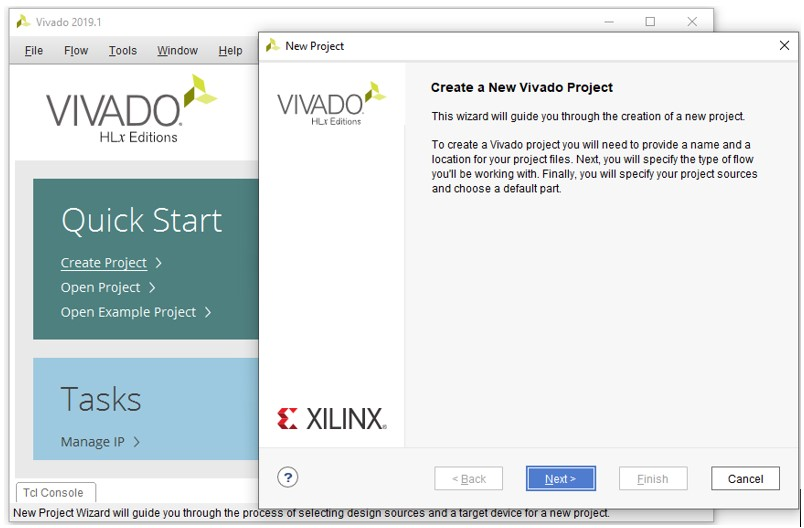
\includegraphics[width=0.5\textwidth]{fig1}
    \caption{Creating a project}
    \label{fig:fig1}
\end{figure}

Next, we need to specify the name and location of the desired project. By clicking the \textbf{Next} button, we move to the next section (Figure~\ref{fig:fig2}).

\begin{figure}[H]
    \centering
    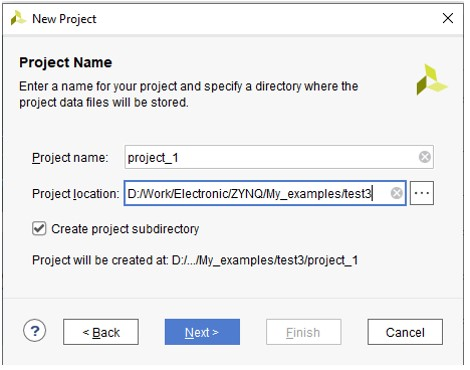
\includegraphics[width=0.5\textwidth]{fig2}
    \caption{Specifying the project name and location}
    \label{fig:fig2}
\end{figure}

In the \textbf{Project Type} section, we select \textbf{RTL Project} as the project type, and by clicking \textbf{Next}, we enter the \textbf{Default Part} section (Figure~\ref{fig:fig3}).

\begin{figure}[H]
    \centering
    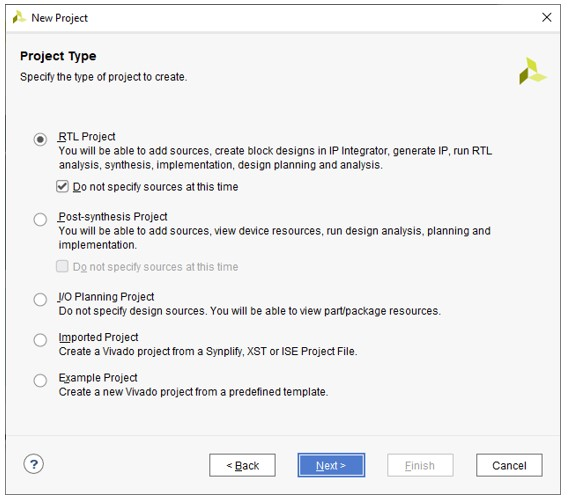
\includegraphics[width=0.5\textwidth]{fig3}
    \caption{Selecting the project type}
    \label{fig:fig3}
\end{figure}

In this window, we must select the target hardware. To make it easier to find the hardware, the filters can be set as shown in the figure, or the part model name can be entered directly in the search box. Since the \textbf{Zynq7010} model is used in this project, the selected part name is \texttt{xc7z010clg400-2} (Figure~\ref{fig:hardware_selection}).

\begin{figure}[H]
    \centering
    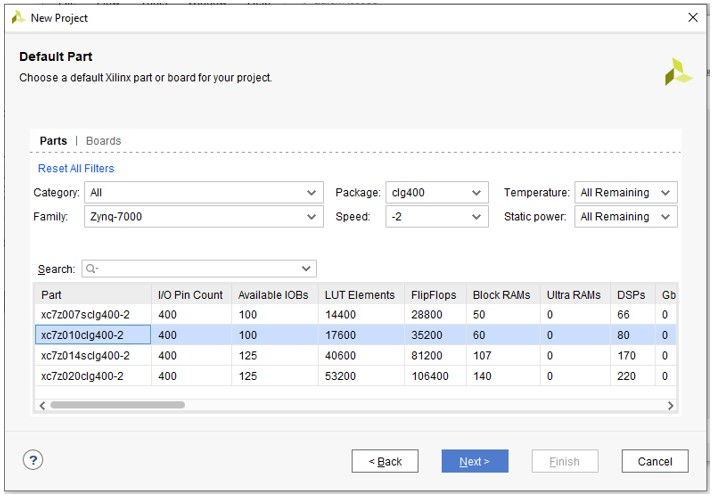
\includegraphics[width=0.5\textwidth]{fig4}
    \caption{Selecting the hardware}
    \label{fig:hardware_selection}
\end{figure}

Again, by clicking the \textbf{Next} button, these settings are applied. After reviewing the displayed information and selecting the \textbf{Finish} button, the steps for creating the new project are completed (Figure~\ref{fig:finish_project_creation}).

\begin{figure}[H]
    \centering
    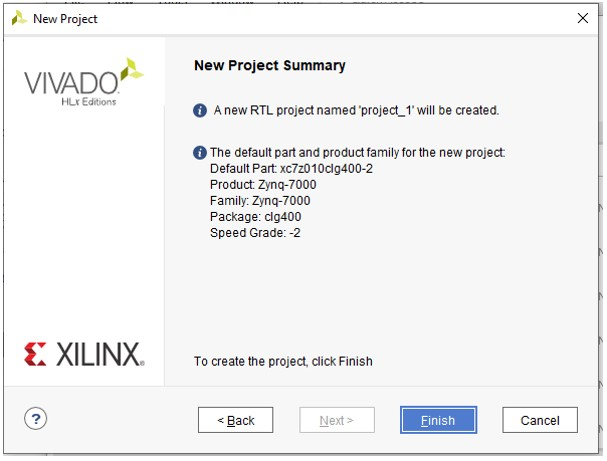
\includegraphics[width=0.5\textwidth]{fig5}
    \caption{Completing the project creation steps}
    \label{fig:finish_project_creation}
\end{figure}

\subsubsection{Adding the Code and Related Sources to the Project}

After creating the project, we enter the Vivado environment. To add a Hardware Description Language (\textbf{HDL}) code, from the \textbf{Sources} section, we click the \textbf{Add Sources} button (Figure~\ref{fig:sources_list}).

\begin{figure}[H]
    \centering
    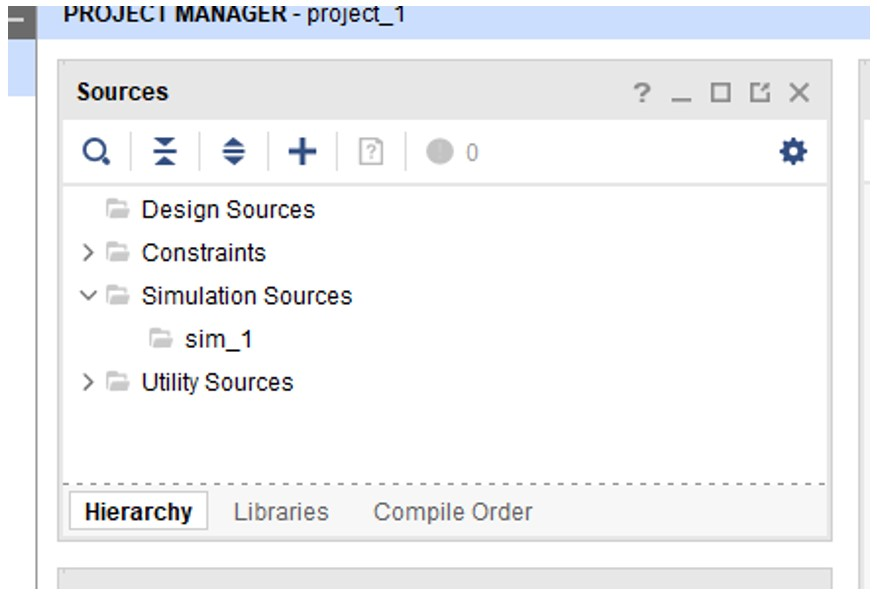
\includegraphics[width=0.5\textwidth]{fig6}
    \caption{List of available sources}
    \label{fig:sources_list}
\end{figure}

In the opened window, we enable the second option, \textbf{Add or create design sources}, if it is disabled, and by clicking \textbf{Next}, we move to the next section (Figure~\ref{fig:create_new_source}).

\begin{figure}[H]
    \centering
    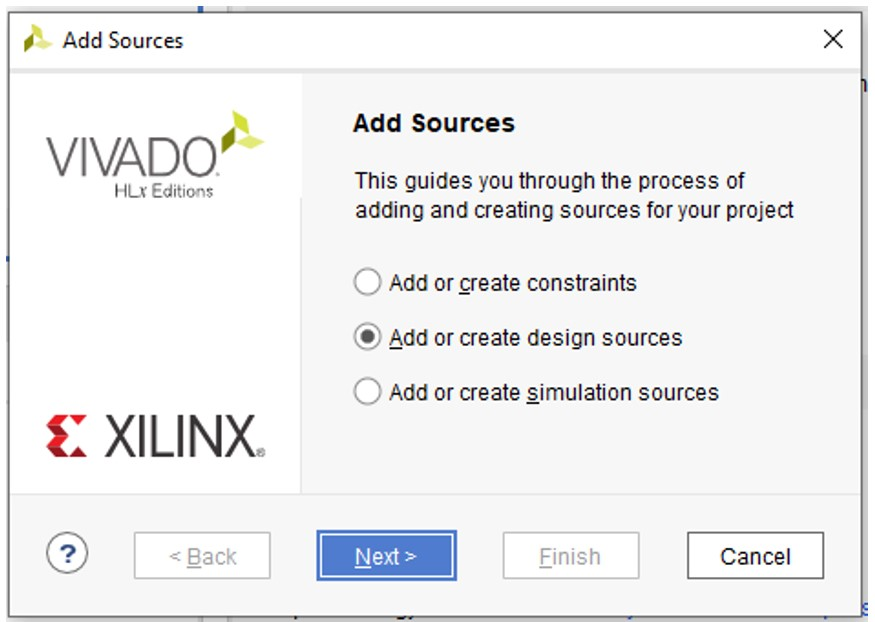
\includegraphics[width=0.5\textwidth]{fig7}
    \caption{Creating a new source}
    \label{fig:create_new_source}
\end{figure}

In this section, to create a new source, we select the \textbf{Create File} button. In the opened window, we choose the desired hardware description language (for example, \textbf{Verilog}) and also specify a name for the source (Figure~\ref{fig:source_name_language}).

\begin{figure}[H]
    \centering
    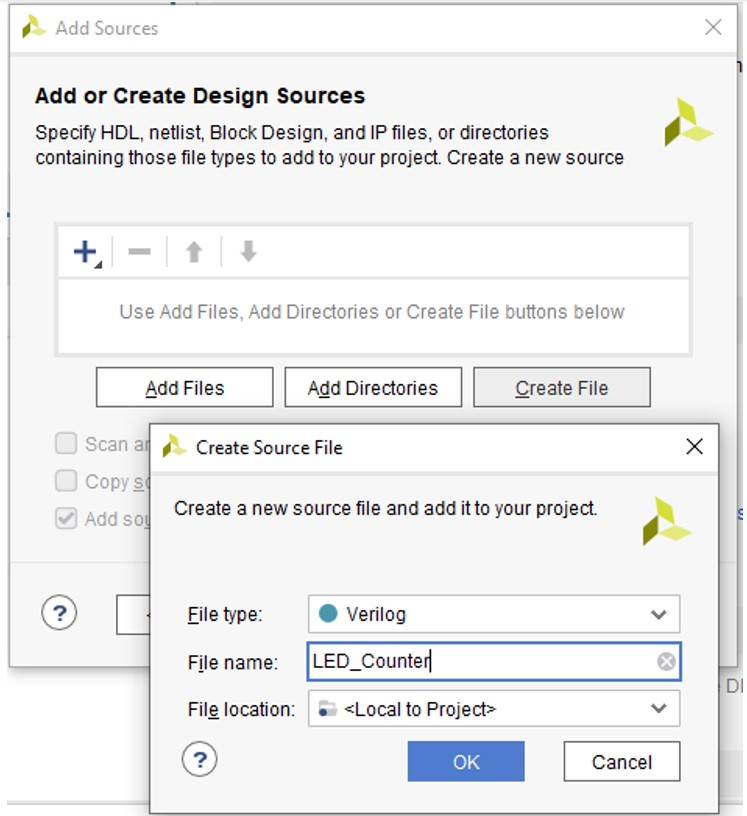
\includegraphics[width=0.5\textwidth]{fig8}
    \caption{Specifying the source name and hardware description language}
    \label{fig:source_name_language}
\end{figure}

If the \textbf{Define Module} window appears, we choose the \textbf{OK} button (Figure~\ref{fig:define_module}).

\begin{figure}[H]
    \centering
    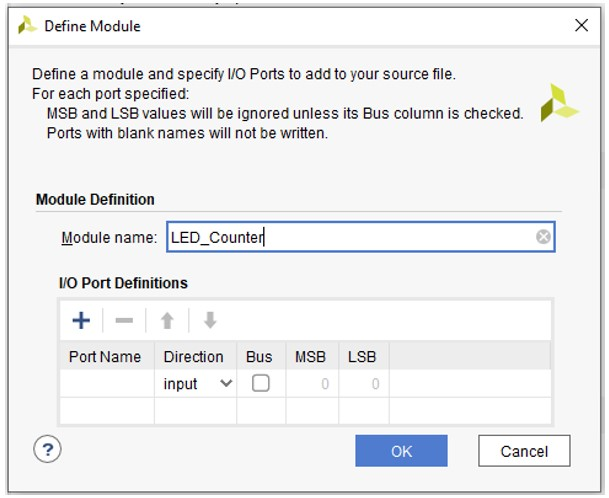
\includegraphics[width=0.5\textwidth]{fig9}
    \caption{Define Module window}
    \label{fig:define_module}
\end{figure}

It can be seen that a file with the \texttt{.v} format (Verilog), with the name chosen in the previous steps, is created under the \textbf{Design Sources} section. By double-clicking on it, its code can be edited. For example, the following code is written in this file to implement a 5-bit counter circuit.

%\paragraph{Code 1: Verilog code for the 5-bit counter}
\begin{lstlisting}[language=Verilog, caption={5-bit counter Verilog code}, label={lst:counter}]
`timescale 1ns / 1ps

module LED_Counter(input clk, output reg [4:0] LED);
reg [31:0] cnt;
always @(posedge clk) begin
    cnt = cnt + 1;
    if(cnt == 25_000_000) begin
        cnt = 0;
        LED = LED + 1;
    end
end
endmodule

\end{lstlisting}



Now it is necessary to assign each signal in the Verilog code to the hardware pins. For this purpose, once again from the \textbf{Sources} section, we click the + button, and this time in the opened window, we select the first option, \textbf{Add or create constraints}, and by clicking \textbf{Next}, we move to the next step (Figure~\ref{fig:create_constraint_file}).


\begin{figure}[H]
    \centering
    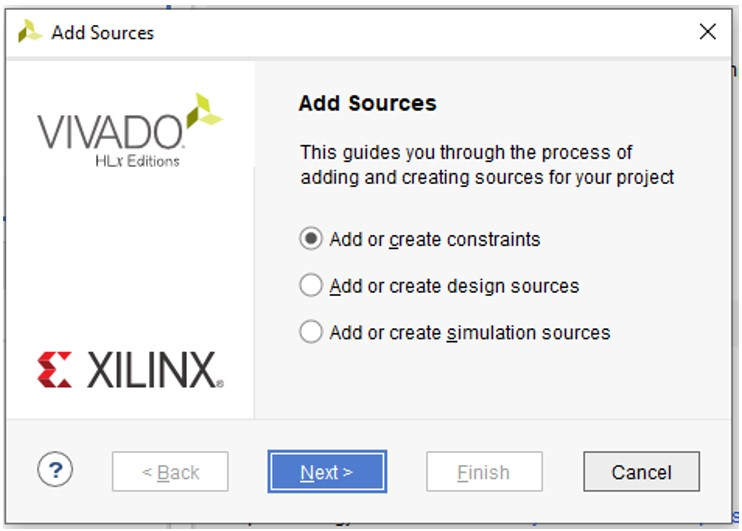
\includegraphics[width=0.5\textwidth]{fig10}
    \caption{Creating the constraint file}
    \label{fig:create_constraint_file}
\end{figure}

In the opened window, we first click the \textbf{Create File} button, then choose a name for the file, and by selecting \textbf{OK} and then \textbf{Finish}, the file is created (Figure~\ref{fig:constraint_file_name}).

\begin{figure}[H]
    \centering
    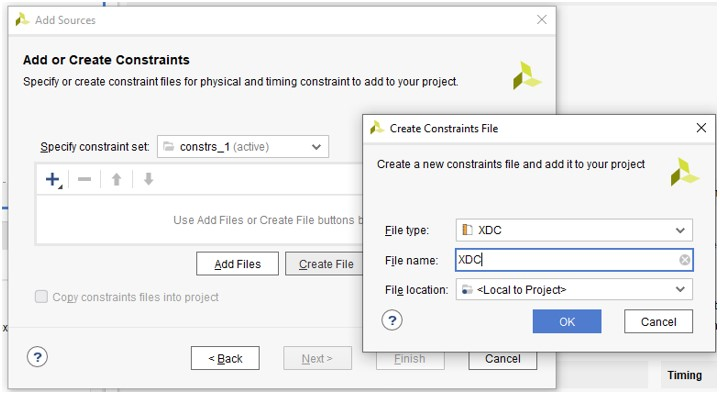
\includegraphics[width=0.5\textwidth]{fig11}
    \caption{Entering the constraint file name}
    \label{fig:constraint_file_name}
\end{figure}

It can be seen that a file with the \texttt{.xdc} format has been created (Figure~\ref{fig:required_files_list}).

\begin{figure}[H]
    \centering
    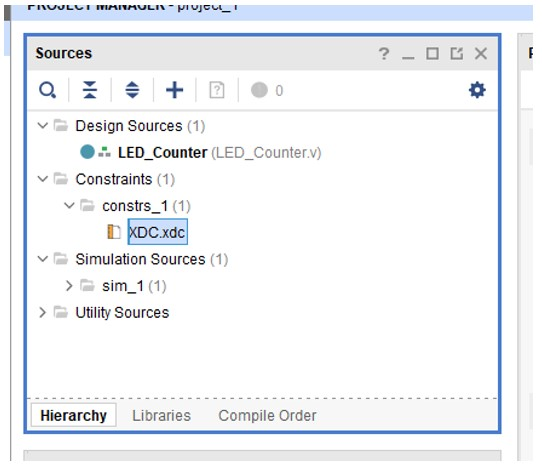
\includegraphics[width=0.5\textwidth]{fig12}
    \caption{Displaying the list of required files}
    \label{fig:required_files_list}
\end{figure}

By double-clicking on this file, we edit it. In the following code, first we set the port standard to \textbf{LVCMOS33}. Then, using the \texttt{PACKAGE\_PIN} parameter, we assign pins to each signal. These pins correspond to the board used in this project.

\begin{lstlisting}[caption={Constraint file for pin assignment}, label={lst:xdc}]
set_property IOSTANDARD LVCMOS33 [get_ports clk]
set_property PACKAGE_PIN U18 [get_ports clk]

set_property IOSTANDARD LVCMOS33 [get_ports {LED[0]}]
set_property PACKAGE_PIN V20 [get_ports {LED[0]}]

set_property IOSTANDARD LVCMOS33 [get_ports {LED[1]}]
set_property PACKAGE_PIN W19 [get_ports {LED[1]}]

set_property IOSTANDARD LVCMOS33 [get_ports {LED[2]}]
set_property PACKAGE_PIN W18 [get_ports {LED[2]}]

set_property IOSTANDARD LVCMOS33 [get_ports {LED[3]}]
set_property PACKAGE_PIN V18 [get_ports {LED[3]}]

set_property IOSTANDARD LVCMOS33 [get_ports {LED[4]}]
set_property PACKAGE_PIN V17 [get_ports {LED[4]}]

\end{lstlisting}

\begin{figure}[H]
    \centering
    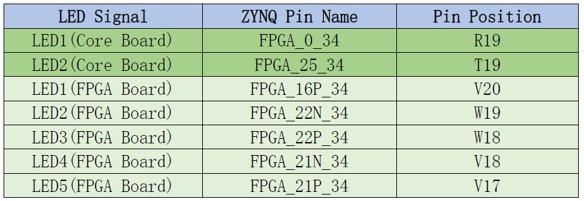
\includegraphics[width=0.5\textwidth]{fig13}
    \caption{Pin names}
    \label{fig:required_files_list}
\end{figure}

It should be noted that the \textbf{PL clock}, which is \textbf{50~MHz}, is connected to pin \texttt{U18}.

\subsubsection{Downloading onto the Hardware}

Now we discuss how to load the written code onto the device and configure it. For this, the code must first be synthesized (\textbf{Synthesis}), implemented (\textbf{Implementation}), and then its \textbf{Bitstream} must be generated and loaded onto the device.

For this purpose, as shown in Figure~\ref{fig:run_synthesis}, we click \textbf{Run Synthesis} and wait until the synthesis process is completed.

\begin{figure}[H]
    \centering
    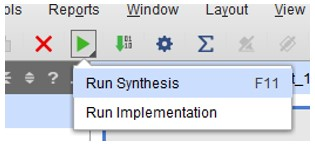
\includegraphics[width=0.5\textwidth]{fig14}
    \caption{Running synthesis}
    \label{fig:run_synthesis}
\end{figure}

Then the next window appears, indicating the completion of the synthesis stage. Now, by selecting \textbf{Run Implementation} and clicking \textbf{OK}, the implementation process begins, and again we must wait until it is completed (Figure~\ref{fig:run_implementation}).

\begin{figure}[H]
    \centering
    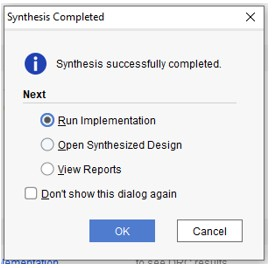
\includegraphics[width=0.5\textwidth]{fig15}
    \caption{Starting implementation after synthesis}
    \label{fig:run_implementation}
\end{figure}

After the following window appears, we select \textbf{Generate Bitstream}, and by clicking \textbf{OK}, the bitstream generation process begins (Figure~\ref{fig:generate_bitstream}).

\begin{figure}[H]
    \centering
    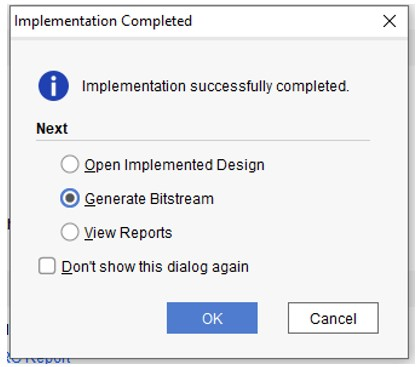
\includegraphics[width=0.5\textwidth]{fig16}
    \caption{Generating the bitstream}
    \label{fig:generate_bitstream}
\end{figure}

Now, we connect the computer to the board's \textbf{JTAG} port using the interface cable and turn on the board. From the \textbf{Flow Navigator} menu on the left side, in the \textbf{PROGRAM AND DEBUG} section, we select \textbf{Open Hardware Manager}, then click \textbf{Open Target} and choose \textbf{Auto Connect} (Figure~\ref{fig:open_hardware_manager}).

\begin{figure}[H]
    \centering
    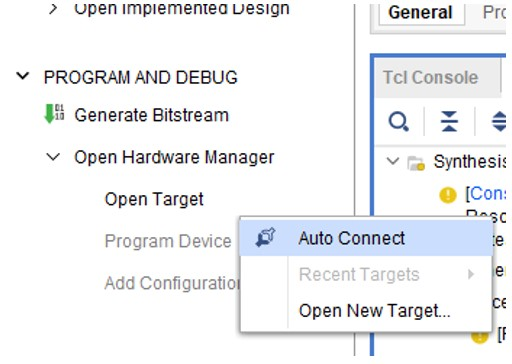
\includegraphics[width=0.5\textwidth]{fig17}
    \caption{Opening Hardware Manager and connecting to the target}
    \label{fig:open_hardware_manager}
\end{figure}

Then, as shown in Figure~\ref{fig:recognized_device}, it can be seen that the device has been recognized by the computer. To send the configuration to the hardware, we click \textbf{Program Device}.

\begin{figure}[H]
    \centering
    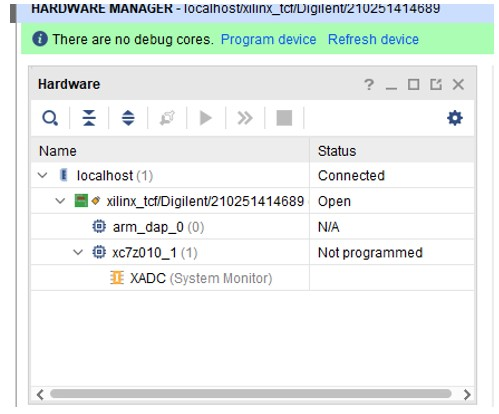
\includegraphics[width=0.5\textwidth]{fig18}
    \caption{Recognized device in Hardware Manager}
    \label{fig:recognized_device}
\end{figure}

In the opened window, we click \textbf{Program} so that the device is configured (Figure~\ref{fig:program_device}).

\begin{figure}[H]
    \centering
    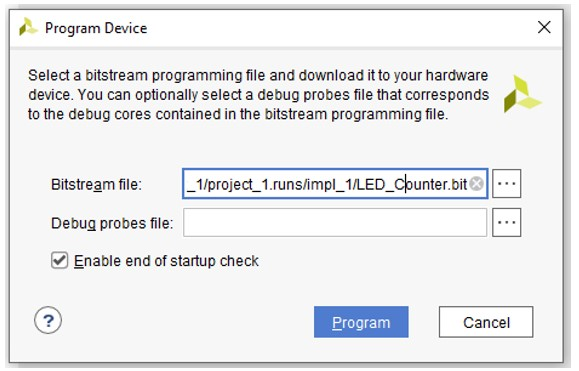
\includegraphics[width=0.5\textwidth]{fig19}
    \caption{Programming the device}
    \label{fig:program_device}
\end{figure}

Now it can be observed that the LEDs on the board turn on and off as a binary counter, as shown in Figure~\ref{fig:counter_output}.

\begin{figure}[H]
    \centering
    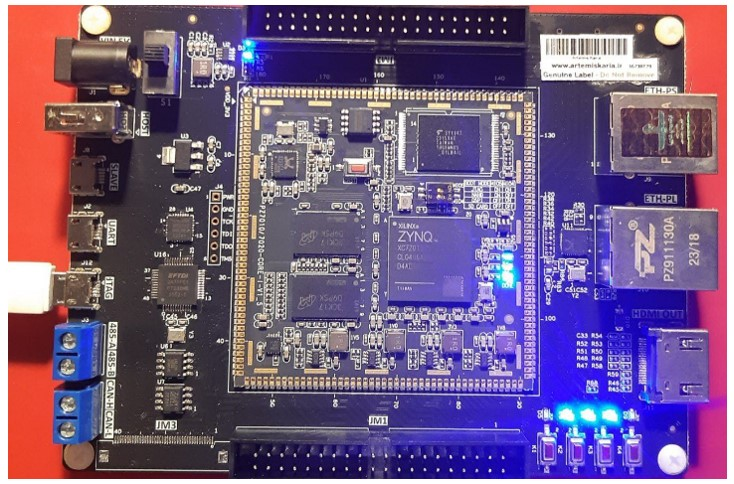
\includegraphics[width=0.5\textwidth]{fig20}
    \caption{5-bit binary counter output on the LEDs}
    \label{fig:counter_output}
\end{figure}


\subsection{MicroBlaze Beside a Custom Hardware}

After creating the project, in the left menu under the \textbf{IP INTEGRATOR} section, click on \textbf{Create Block Design} (Figure~\ref{fig:fig26}).

\begin{figure}[H]
    \centering
    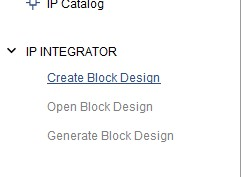
\includegraphics[width=0.5\textwidth]{fig26}
    \caption{Creating a new block design}
    \label{fig:fig26}
\end{figure}

In the displayed window, after setting a name such as \texttt{design\_1}, click the \textbf{OK} button to create an empty block design. In this window, click the \textbf{+} button and search for \textbf{MicroBlaze} to add it to the block design. For now, we leave the MicroBlaze settings at their default values (Figure~\ref{fig:fig27}).

\begin{figure}[H]
    \centering
    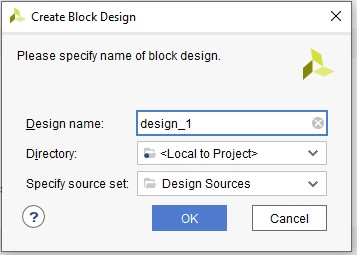
\includegraphics[width=0.5\textwidth]{fig27}
    \caption{Adding MicroBlaze to the block design}
    \label{fig:fig27}
\end{figure}

After adding MicroBlaze, click \textbf{Run Block Automation} at the top of the block design window (Figure~\ref{fig:fig28}).

\begin{figure}[H]
    \centering
    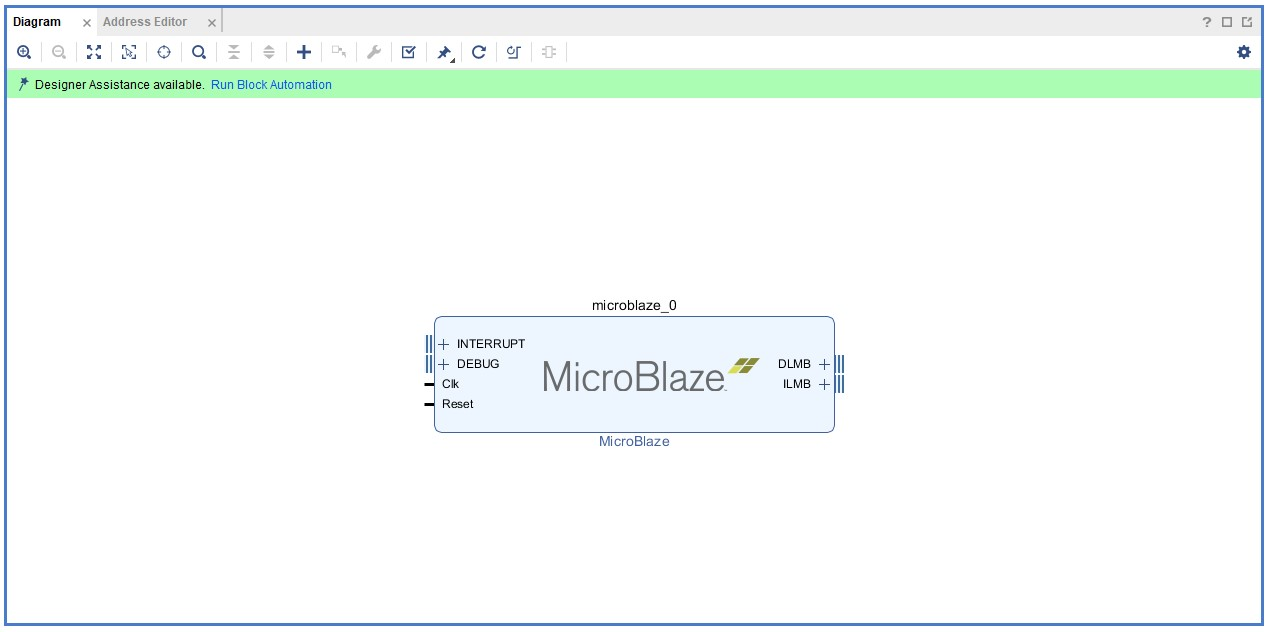
\includegraphics[width=0.5\textwidth]{fig28}
    \caption{Running block automation for MicroBlaze}
    \label{fig:fig28}
\end{figure}

In the displayed window, leave the parameters at their default values and, for the clock connection, choose the \textbf{New External Port} option (Figure~\ref{fig:fig29}).

\begin{figure}[H]
    \centering
    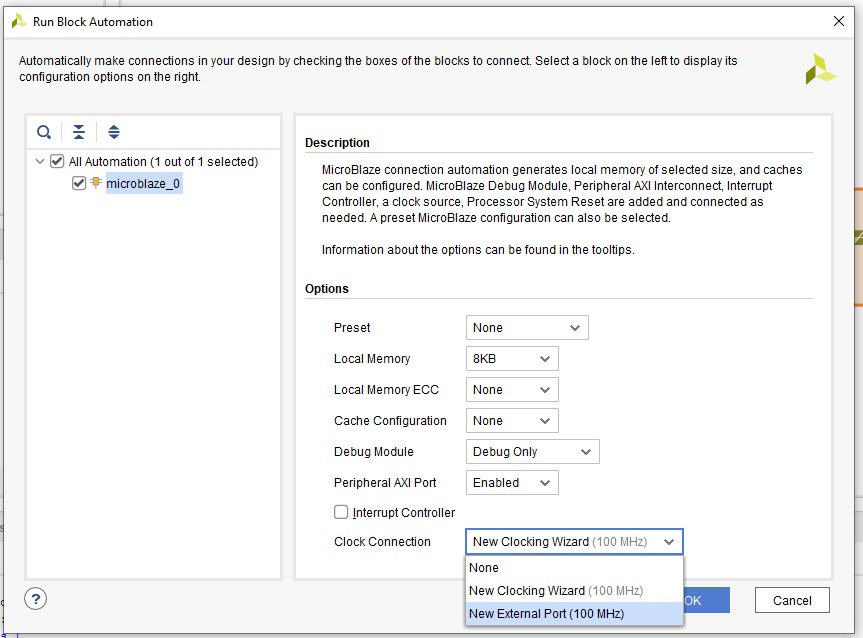
\includegraphics[width=0.5\textwidth]{fig29}
    \caption{Configuring block automation settings}
    \label{fig:fig29}
\end{figure}

As shown, several blocks will appear, including local memory, a debug module, and other required components (Figure~\ref{fig:fig30}).

\begin{figure}[H]
    \centering
    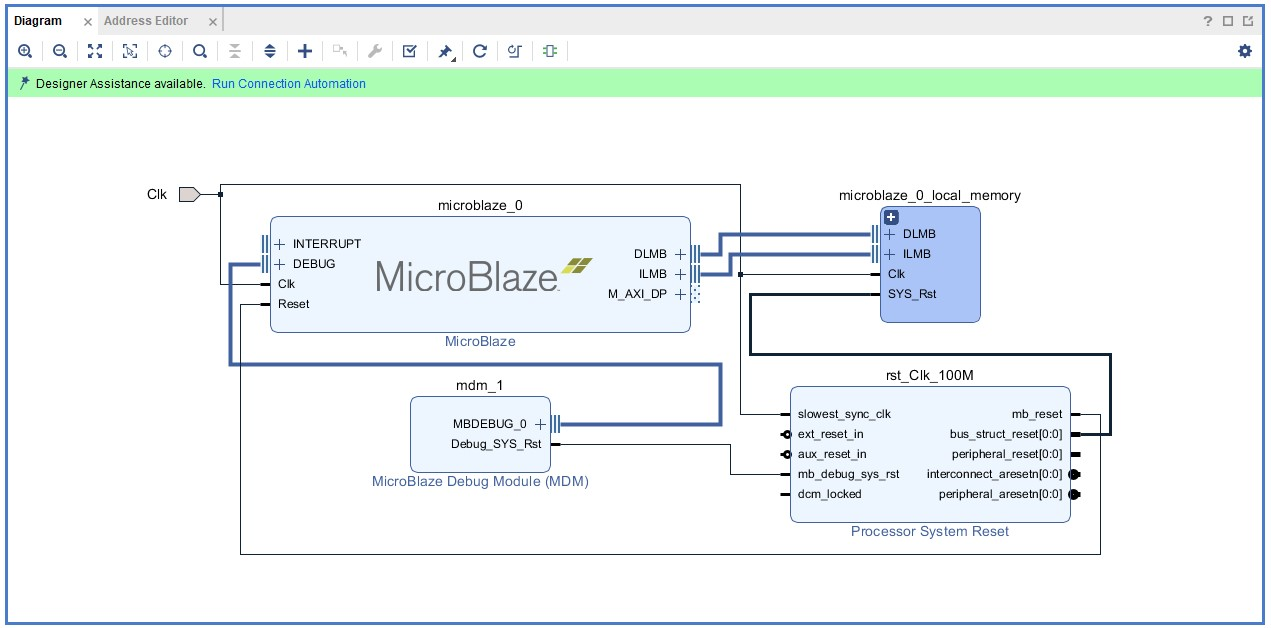
\includegraphics[width=0.5\textwidth]{fig30}
    \caption{Automatically generated MicroBlaze system components}
    \label{fig:fig30}
\end{figure}

Again, click \textbf{Run Block Automation} at the top of the block design window. In the following window, for the reset connection, choose \textbf{New External Port}. According to the development board datasheet, the reset signal is pulled up to the 3.3\,V power source, so the reset type should be selected as \textbf{ACTIVE\_LOW} in this case (Figure~\ref{fig:fig31}).

\begin{figure}[H]
    \centering
    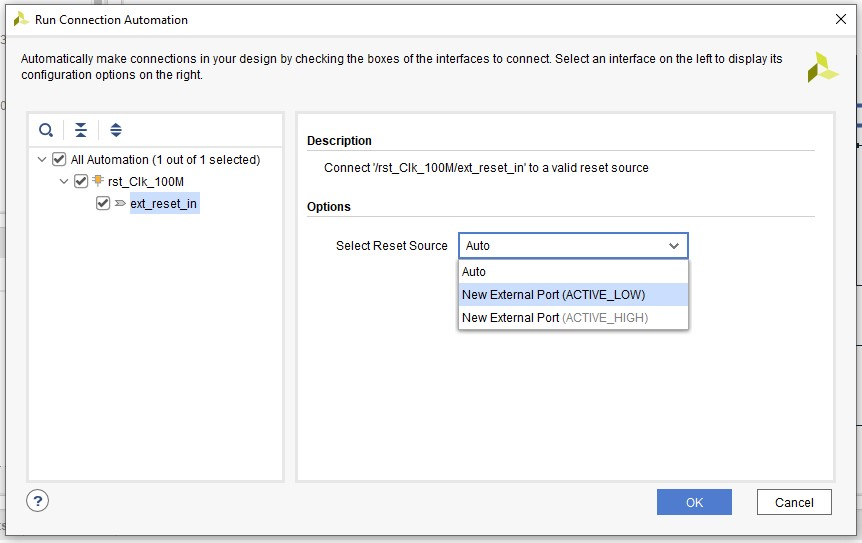
\includegraphics[width=0.5\textwidth]{fig31}
    \caption{Configuring the external reset port}
    \label{fig:fig31}
\end{figure}

After this step, as shown, in addition to the clock port that was set as an external port, the system reset signal (\texttt{reset\_rtl\_0}) is also set as an external port. Then, click the \textbf{Validate Design} button or press the shortcut key \textbf{F6} to validate the design and check whether any errors occur (Figure~\ref{fig:fig32}).

\begin{figure}[H]
    \centering
    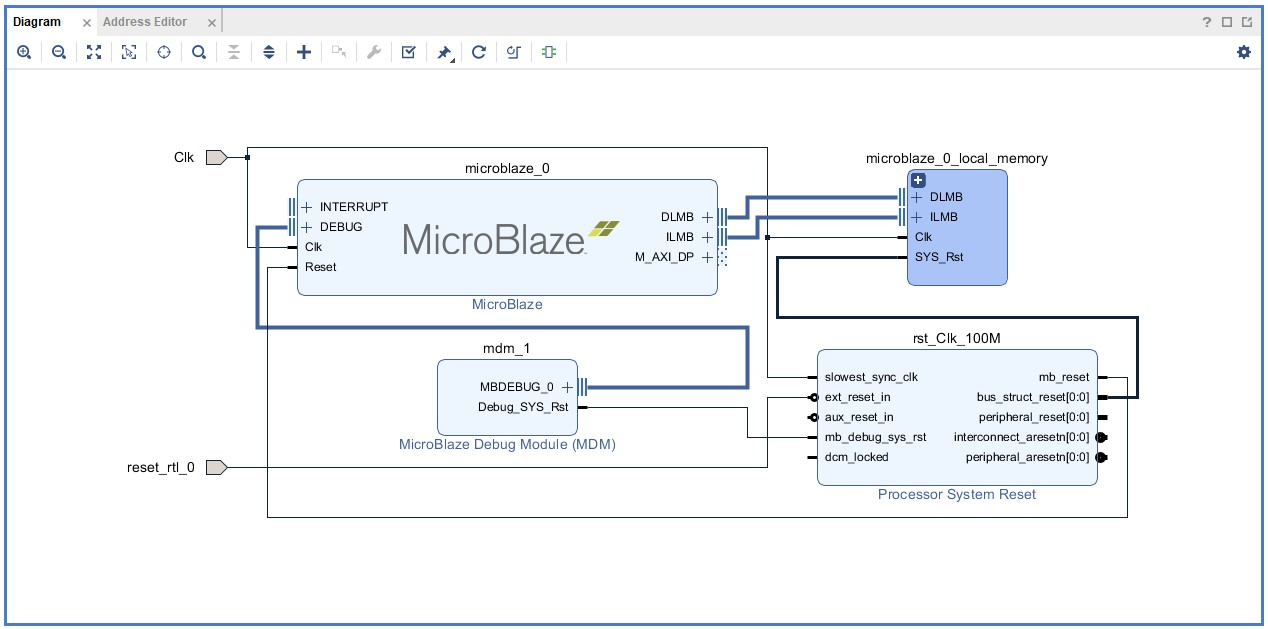
\includegraphics[width=0.5\textwidth]{fig32}
    \caption{Validating the block design}
    \label{fig:fig32}
\end{figure}

\subsubsection{Adding Custom Hardware}

In this case, we want to add our custom hardware to the design. For simplicity, we will create a simple adder as our custom hardware. For this purpose, from the top menu bar, go to \textbf{Tools} and select \textbf{Create and Package New IP} (Figure~\ref{fig:fig33}).

\begin{figure}[H]
    \centering
    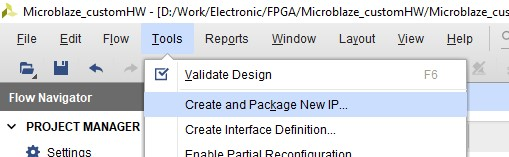
\includegraphics[width=0.5\textwidth]{fig33}
    \caption{Opening the Create and Package New IP tool}
    \label{fig:fig33}
\end{figure}

In the displayed tab titled \textbf{Create and Package New IP}, click \textbf{Next} to begin the process (Figure~\ref{fig:fig34}).

\begin{figure}[H]
    \centering
    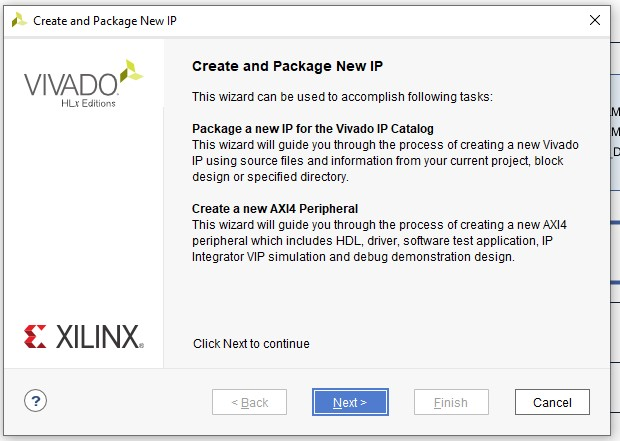
\includegraphics[width=0.5\textwidth]{fig34}
    \caption{Starting the IP packaging process}
    \label{fig:fig34}
\end{figure}

Because we are using the MicroBlaze soft-core processor, which uses AXI interconnect as the standard interconnection protocol, in order to connect our custom hardware to MicroBlaze, we must choose the \textbf{Create a new AXI4 peripheral} option (Figure~\ref{fig:fig35}).

\begin{figure}[H]
    \centering
    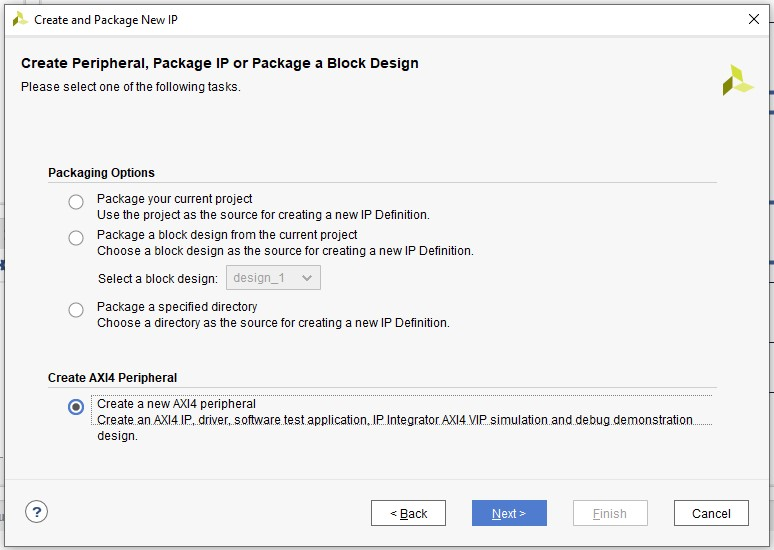
\includegraphics[width=0.5\textwidth]{fig35}
    \caption{Selecting AXI4 peripheral creation}
    \label{fig:fig35}
\end{figure}

Here, we can modify the details of our custom hardware, such as its name and version. For this example, we leave \texttt{myip} as the name and keep the other options unchanged (Figure~\ref{fig:fig36}).

\begin{figure}[H]
    \centering
    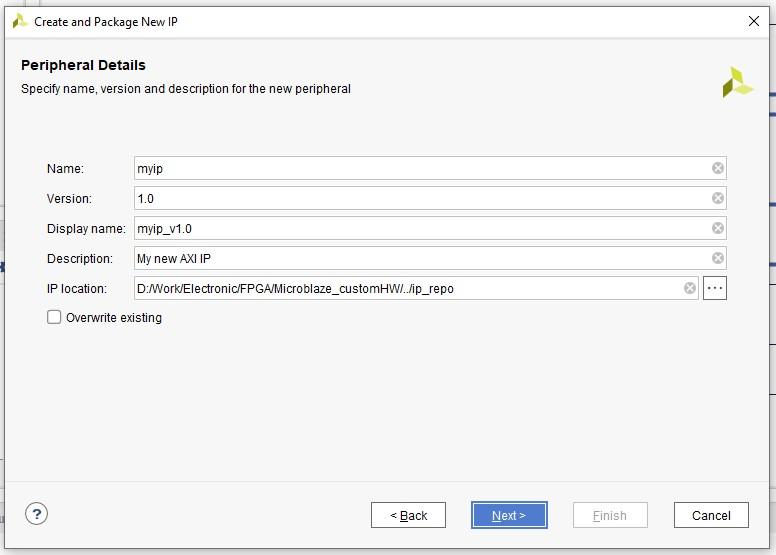
\includegraphics[width=0.5\textwidth]{fig36}
    \caption{Setting the custom IP name and properties}
    \label{fig:fig36}
\end{figure}

In the \textbf{Add Interfaces} step, we should define the interconnect through which our custom hardware communicates with other peripherals or hardware modules, especially the processor. For this purpose, we keep the name of this interconnect port as \texttt{S00\_AXI} for our custom IP. We choose the interface type and mode as \textbf{Lite} and \textbf{Slave}, respectively, with a 32-bit data width. The important option here is the number of registers, because these registers play a key role in sharing data between MicroBlaze and the custom hardware. Here, we choose 4 registers because we are implementing an adder, and we can map the two input ports and the output to three separate registers. One register will remain unused (Figure~\ref{fig:fig37}).

\begin{figure}[H]
    \centering
    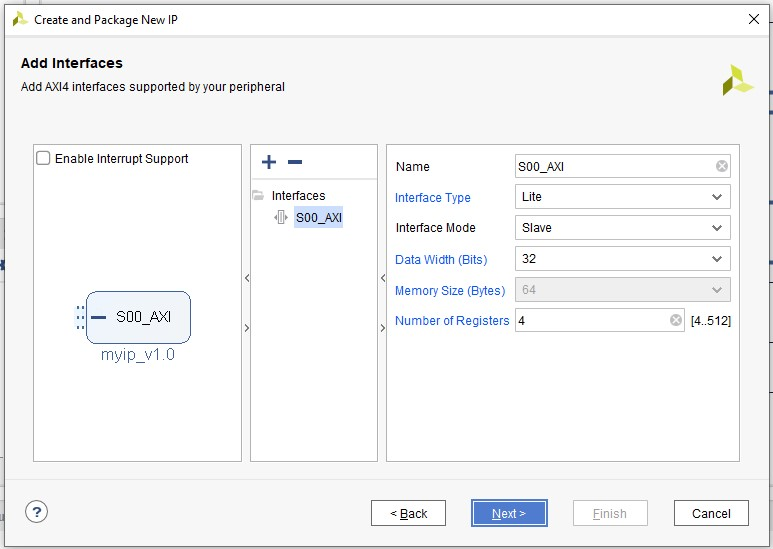
\includegraphics[width=0.5\textwidth]{fig37}
    \caption{Configuring the AXI interface and registers}
    \label{fig:fig37}
\end{figure}

Finally, we choose \textbf{Add IP to Repository} and click the \textbf{Finish} button (Figure~\ref{fig:fig38}).

\begin{figure}[H]
    \centering
    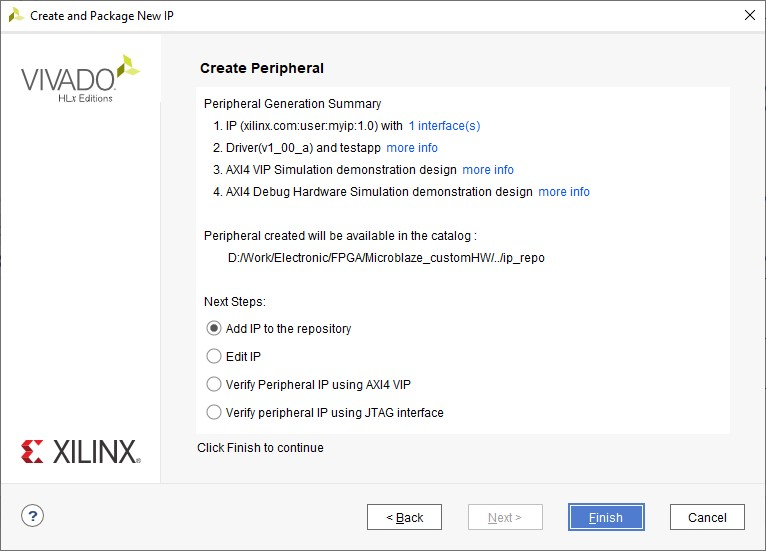
\includegraphics[width=0.5\textwidth]{fig38}
    \caption{Adding the custom IP to the repository}
    \label{fig:fig38}
\end{figure}

Now we can add the created custom IP to the block design. To do this, just like adding other IPs, we press the \textbf{+} button and search for our custom hardware name, which is \texttt{myip} (Figure~\ref{fig:fig39}).

\begin{figure}[H]
    \centering
    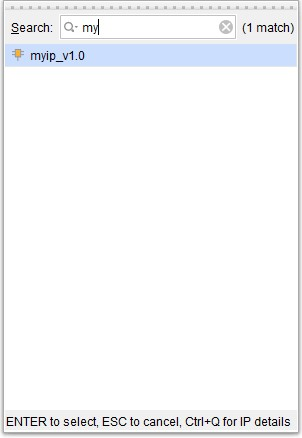
\includegraphics[width=0.5\textwidth]{fig39}
    \caption{Adding the custom IP to the block design}
    \label{fig:fig39}
\end{figure}
In order to describe our custom IP, right-click on the added IP in the block design window and choose \textbf{Edit in IP Packager} (Figure~\ref{fig:fig40}).

\begin{figure}[H]
    \centering
    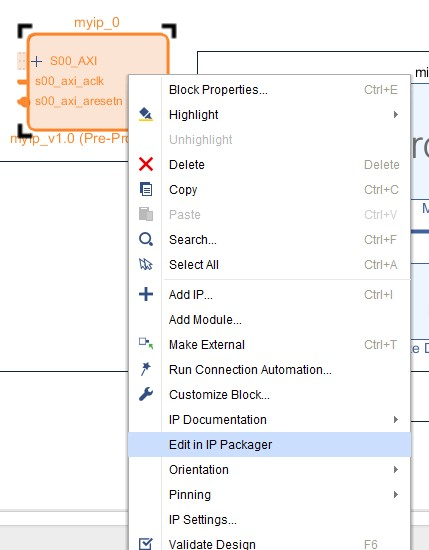
\includegraphics[width=0.5\textwidth]{fig40}
    \caption{Opening the custom IP in the IP Packager}
    \label{fig:fig40}
\end{figure}

In the following window, click \textbf{OK} (Figure~\ref{fig:fig41}).

\begin{figure}[H]
    \centering
    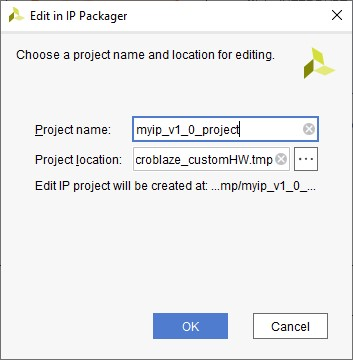
\includegraphics[width=0.5\textwidth]{fig41}
    \caption{Confirming the IP Packager launch}
    \label{fig:fig41}
\end{figure}

A new Vivado window will appear. This new window is related to the custom hardware. In the \textbf{Sources} section, under the \textbf{Hierarchy} tab, double-click on \texttt{myip\_v1\_0\_S00\_AXI\_Inst} to modify it (Figure~\ref{fig:fig42}). As a result, the generated template code will be displayed, which already contains the AXI interconnect logic. To define our own circuit, scroll down until you see the comment \texttt{// Add user logic here}, and write the required logic in that section.

Since we previously defined 4 registers, we can access these registers to read from or write to them. For example, if \texttt{sum\_wire = a + b}, we can map \texttt{a} to \texttt{slv\_reg0}, \texttt{b} to \texttt{slv\_reg1}, and \texttt{sum\_wire} to \texttt{slv\_reg2}. Therefore, our code will be as shown in Listing~\ref{lst:lst1}.

\begin{figure}[H]
    \centering
    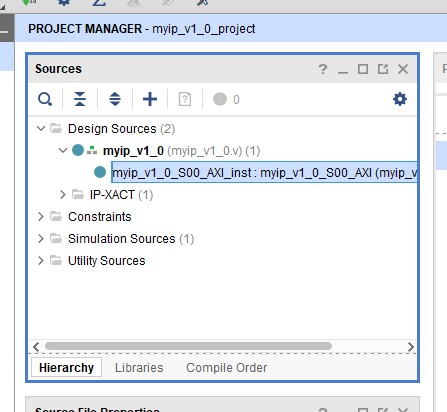
\includegraphics[width=0.5\textwidth]{fig42}
    \caption{Opening the AXI module source file for modification}
    \label{fig:fig42}
\end{figure}

\begin{lstlisting}[language=Verilog, caption={Adding the user logic for the custom adder}, label={lst:lst1}]
    // Add user logic here
    wire [31:0] sum_wire;
    assign sum_wire = slv_reg0 + slv_reg1;
    // User logic ends
\end{lstlisting}

Another required change is in the register read logic. In the following code section, we should replace \texttt{slv\_reg2} with \texttt{sum\_wire}, as shown in line 12 of Listing~\ref{lst:lst2}.

\begin{lstlisting}[language=Verilog, caption={Modifying the AXI read logic to return the adder output}, label={lst:lst2}]
    ...
    // Implement memory mapped register select and read logic generation
    // Slave register read enable is asserted when valid address is available
    // and the slave is ready to accept the read address.
    assign slv_reg_rden = axi_arready & S_AXI_ARVALID & ~axi_rvalid;
    always @(*)
    begin
          // Address decoding for reading registers
          case ( axi_araddr[ADDR_LSB+OPT_MEM_ADDR_BITS:ADDR_LSB] )
            2'h0   : reg_data_out <= slv_reg0;
            2'h1   : reg_data_out <= slv_reg1;
            2'h2   : reg_data_out <= sum_wire;
            2'h3   : reg_data_out <= slv_reg3;
            default : reg_data_out <= 0;
          endcase
    end
    ...
\end{lstlisting}

Finally, to save the changes made to the custom IP, go to the \textbf{Package IP - myip} tab. In the \textbf{Review and Package} section, click \textbf{Re-package IP} to save the changes. Note that if you make other changes, such as adding ports to the Verilog module, you should also apply the corresponding updates in the \textbf{Ports and Interfaces} section (Figure~\ref{fig:fig42_1}).

\begin{figure}[H]
    \centering
    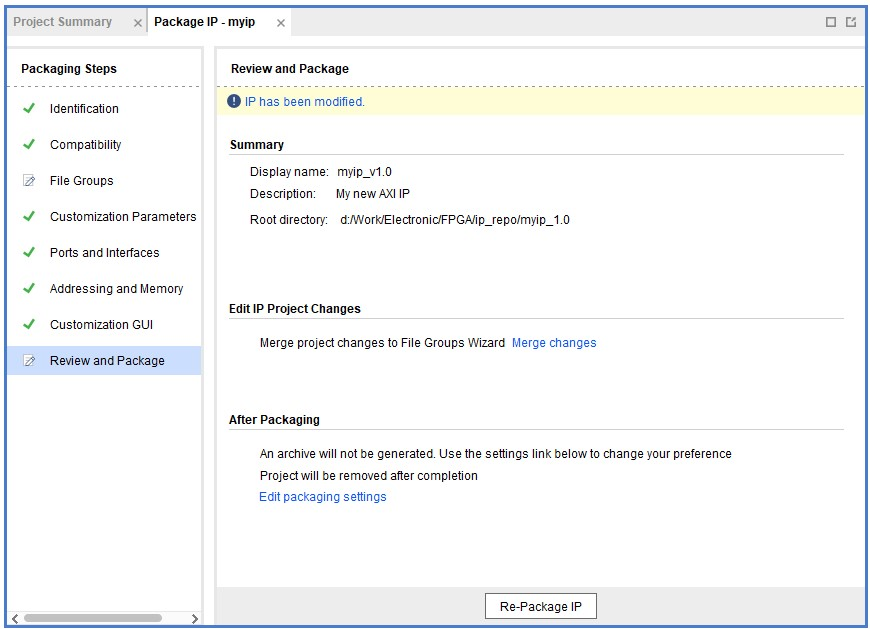
\includegraphics[width=0.5\textwidth]{fig42_1}
    \caption{Re-packaging the custom IP after modification}
    \label{fig:fig42_1}
\end{figure}

In the displayed window, click \textbf{Yes} to close the Vivado window related to the custom IP and return to the main Vivado window (Figure~\ref{fig:fig42_2}).

\begin{figure}[H]
    \centering
    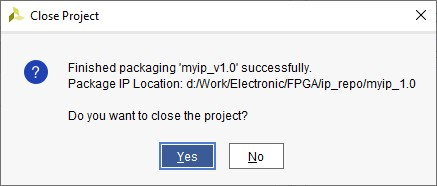
\includegraphics[width=0.5\textwidth]{fig42_2}
    \caption{Confirming closure of the custom IP Vivado window}
    \label{fig:fig42_2}
\end{figure}

After closing the custom IP Vivado window and returning to the main Vivado window, click on \textbf{Refresh IP Catalog} at the top of the window.

\begin{figure}[H]
    \centering
    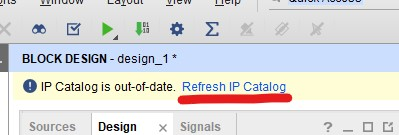
\includegraphics[width=0.5\textwidth]{fig43}
    \caption{Refreshing the IP Catalog}
    \label{fig:fig43}
\end{figure}

After that, in the \textbf{IP Status} section at the bottom of the window, select all IPs and click \textbf{Upgrade Selected}.

\begin{figure}[H]
    \centering
    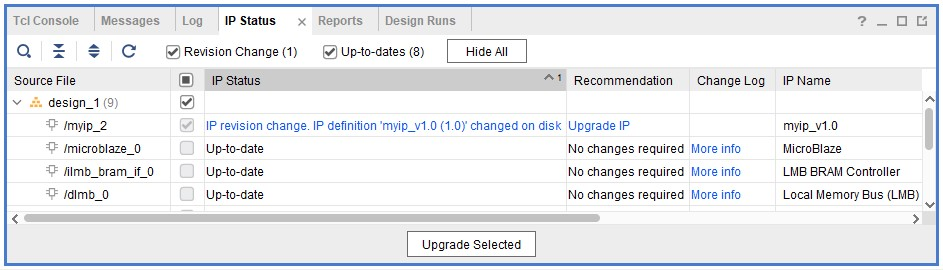
\includegraphics[width=0.5\textwidth]{fig42_3}
    \caption{Upgrading the selected IPs}
    \label{fig:fig42_3}
\end{figure}

If a window titled \textbf{Generate Output Products} appears, click \textbf{Skip}  (Figure~\ref{fig:fig42_4}).

\begin{figure}[H]
    \centering
    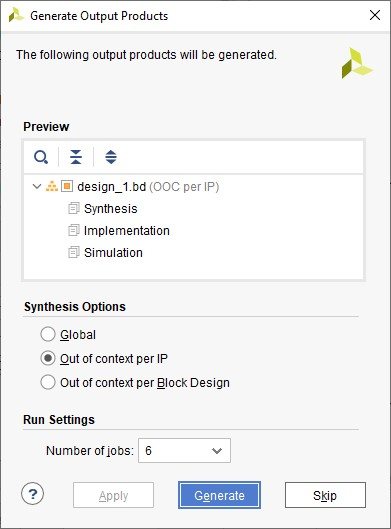
\includegraphics[width=0.5\textwidth]{fig42_4}
    \caption{Skipping output product generation}
    \label{fig:fig42_4}
\end{figure}

Then click \textbf{Run Connection Automation}, which opens a window where we should assign the clock of our custom IP to the clock port that was created previously (\texttt{Clk}) (Figure~\ref{fig:fig44}).

\begin{figure}[H]
    \centering
    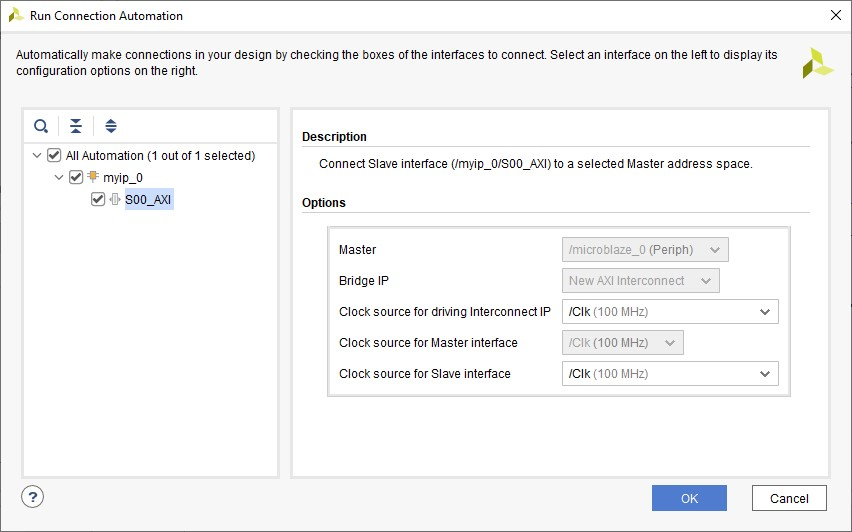
\includegraphics[width=0.5\textwidth]{fig44}
    \caption{Connecting the custom IP clock using automation}
    \label{fig:fig44}
\end{figure}

The complete system block design should be as shown in Figure~\ref{fig:fig44_5}.

\begin{figure}[H]
    \centering
    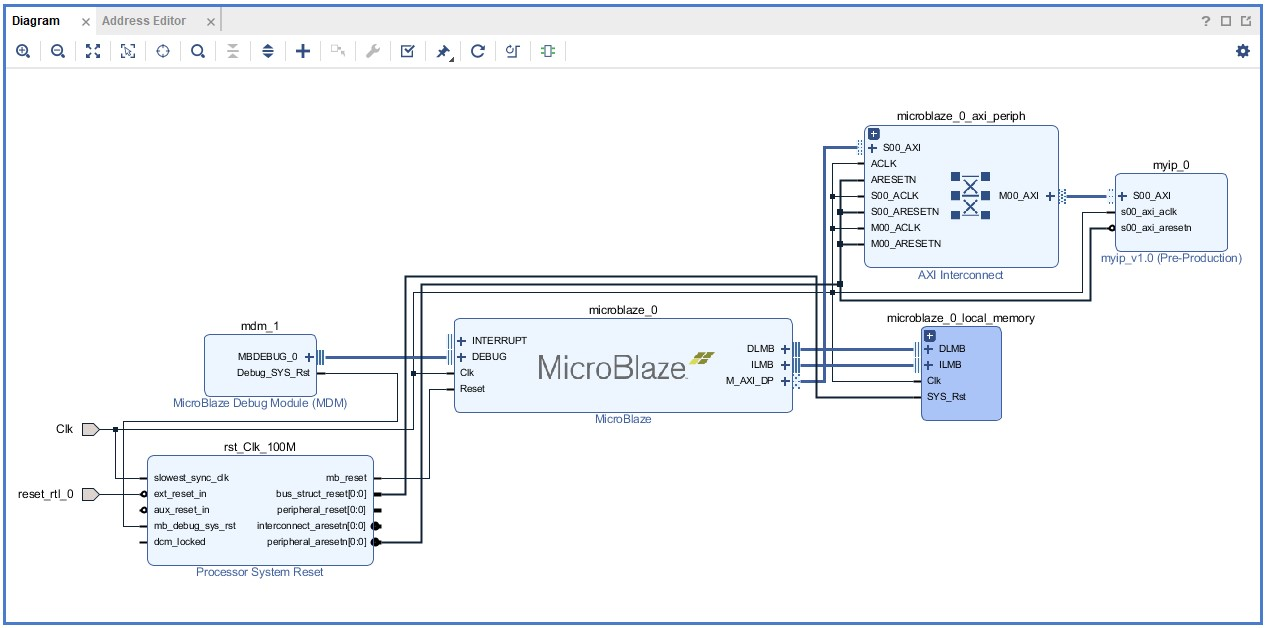
\includegraphics[width=0.7\textwidth]{fig44_5}
    \caption{Complete system block design including MicroBlaze and the custom IP}
    \label{fig:fig44_5}
\end{figure}

In the \textbf{Address Editor} tab, next to the \textbf{Diagram} tab, we can see that our custom hardware has been added and that its address has been assigned automatically so that it can be accessed according to the memory-mapped system structure (Figure~\ref{fig:fig45}).

\begin{figure}[H]
    \centering
    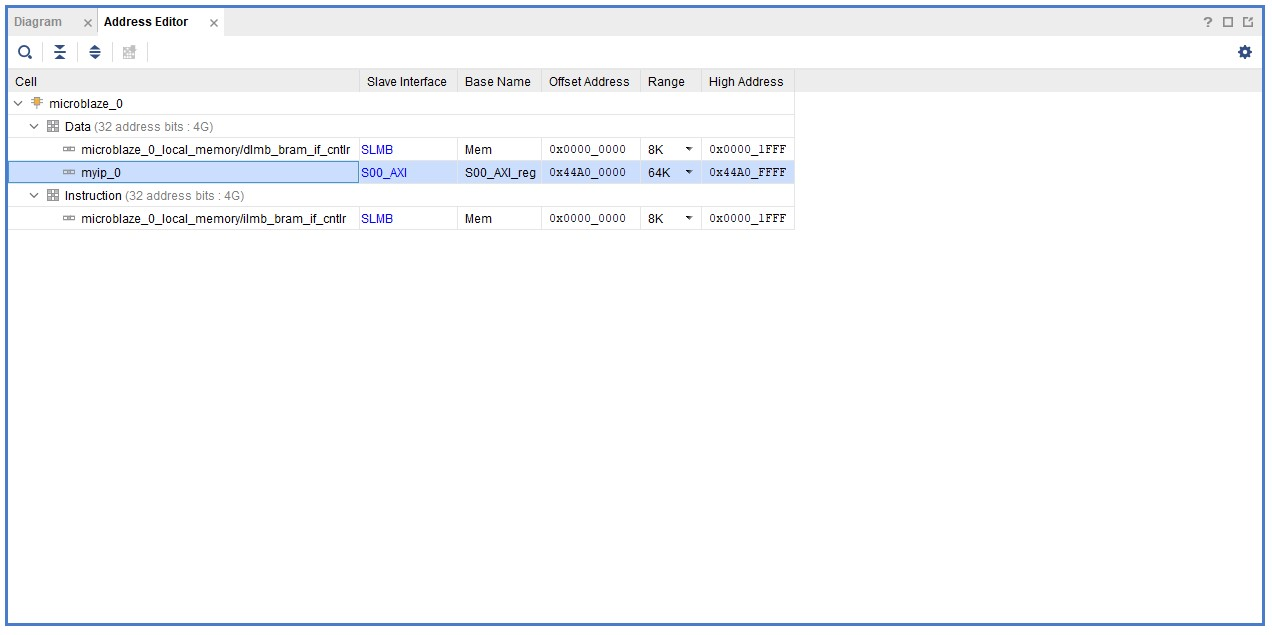
\includegraphics[width=0.5\textwidth]{fig45}
    \caption{Automatically assigned address for the custom hardware}
    \label{fig:fig45}
\end{figure}

Again, by clicking \textbf{Validate Design} in the \textbf{Diagram} tab, we can check whether the whole design is valid and free of errors.


Now it is necessary to assign the top-level signals to the hardware pins. For this purpose, from the \textbf{Sources} section, we click the \textbf{+} button. In the opened window, we select the first option, \textbf{Add or create constraints}, and by clicking \textbf{Next}, we move to the next step (Figure~\ref{fig:fig46} and Figure~\ref{fig:create_constraint_file}).

\begin{figure}[H]
    \centering
    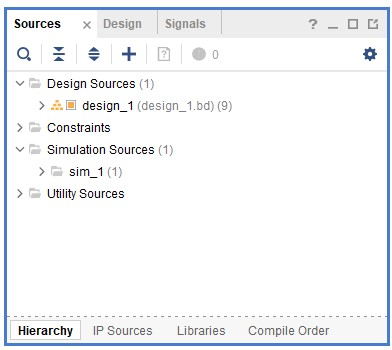
\includegraphics[width=0.5\textwidth]{fig46}
    \caption{Opening the Add Sources window}
    \label{fig:fig46}
\end{figure}

\begin{figure}[H]
    \centering
    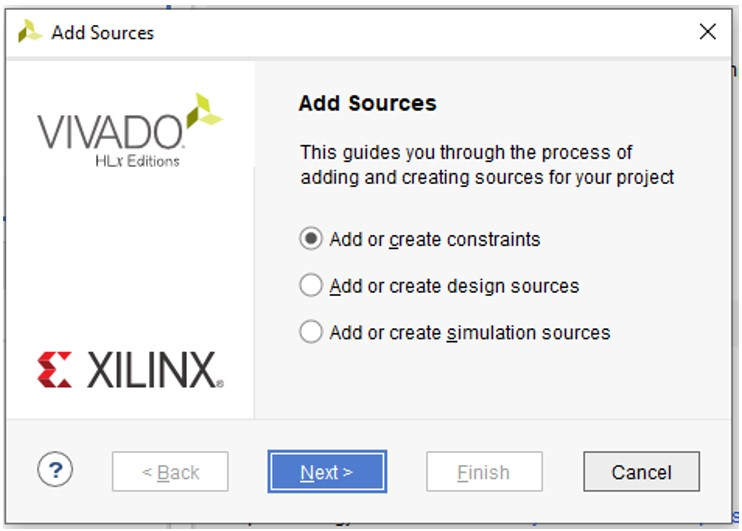
\includegraphics[width=0.5\textwidth]{fig10}
    \caption{Creating the constraint file}
    \label{fig:create_constraint_file}
\end{figure}

In the opened window, we first click the \textbf{Create File} button, then choose a name for the file, and by selecting \textbf{OK} and then \textbf{Finish}, the file is created (Figure~\ref{fig:constraint_file_name}).

\begin{figure}[H]
    \centering
    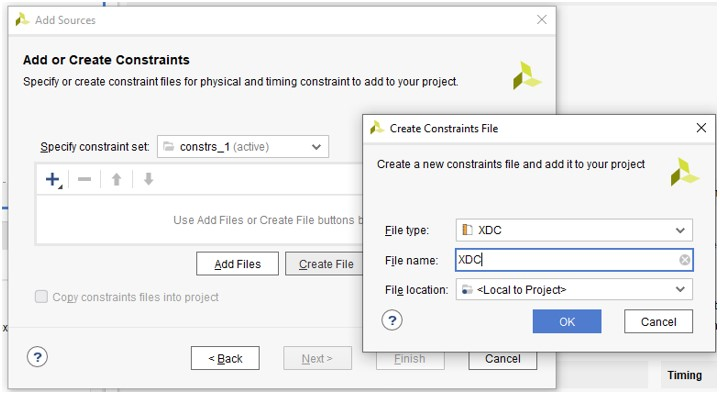
\includegraphics[width=0.5\textwidth]{fig11}
    \caption{Entering the constraint file name}
    \label{fig:constraint_file_name}
\end{figure}

It can be seen that a file with the \texttt{.xdc} format has been created (Figure~\ref{fig:required_files_list}).

\begin{figure}[H]
    \centering
    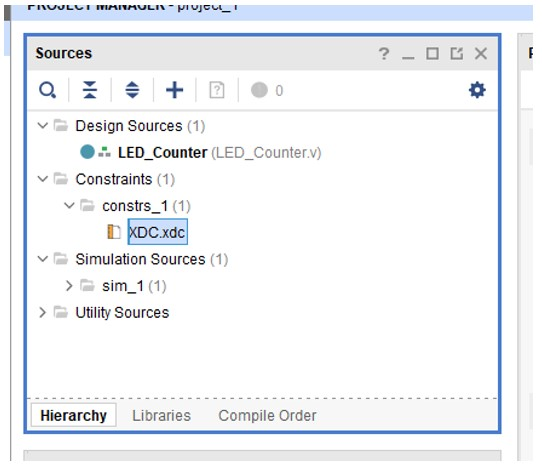
\includegraphics[width=0.5\textwidth]{fig12}
    \caption{Displaying the list of required files}
    \label{fig:required_files_list}
\end{figure}

By double-clicking on this file, we can edit it. In the following code, we assign the top-level ports to the corresponding board pins using the \texttt{PACKAGE\_PIN} parameter and set the I/O standard to \textbf{LVCMOS33}.

\begin{lstlisting}[caption={Constraint file for clock and reset pin assignment}, label={lst:xdc_clk_reset}]
set_property PACKAGE_PIN U19 [get_ports reset_rtl_0]
set_property IOSTANDARD LVCMOS33 [get_ports reset_rtl_0]

set_property PACKAGE_PIN U18 [get_ports Clk]
set_property IOSTANDARD LVCMOS33 [get_ports Clk]
\end{lstlisting}
In the \textbf{Sources} section, right-click on \texttt{design\_1.bd} and select \textbf{Create HDL Wrapper} (Figure~\ref{fig:fig47}). Then select \textbf{Let Vivado manage wrapper and auto-update} and click \textbf{OK}.

\begin{figure}[H]
    \centering
    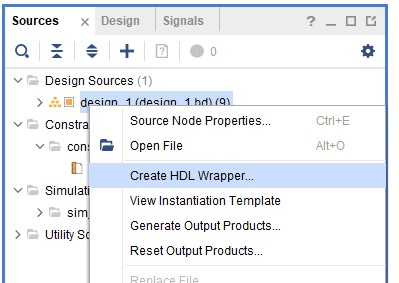
\includegraphics[width=0.5\textwidth]{fig47}
    \caption{Creating an HDL wrapper for the block design}
    \label{fig:fig47}
\end{figure}

\begin{figure}[H]
    \centering
    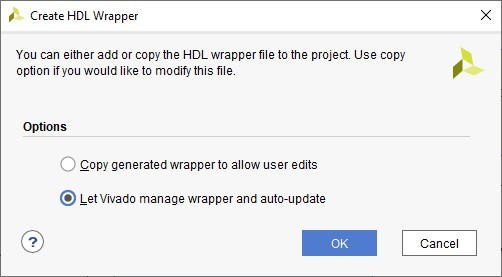
\includegraphics[width=0.5\textwidth]{fig48}
    \caption{Selecting automatic wrapper generation}
    \label{fig:fig48}
\end{figure}

After that, you can see that a wrapper has been created for the block design (Figure~\ref{fig:fig49}).

\begin{figure}[H]
    \centering
    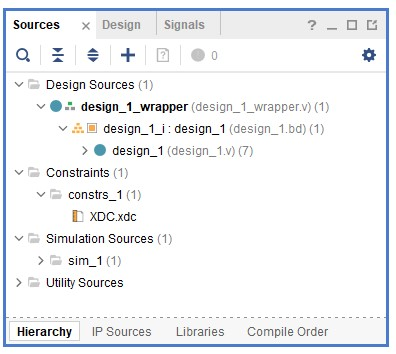
\includegraphics[width=0.5\textwidth]{fig49}
    \caption{Generated HDL wrapper for the block design}
    \label{fig:fig49}
\end{figure}

Now we discuss how to load the written design onto the device and configure it. For this, the design must first be synthesized (\textbf{Synthesis}), implemented (\textbf{Implementation}), and then its \textbf{Bitstream} must be generated and loaded onto the device.

For this purpose, as shown in Figure~\ref{fig:run_synthesis}, we click \textbf{Run Synthesis} and wait until the synthesis process is completed.

\begin{figure}[H]
    \centering
    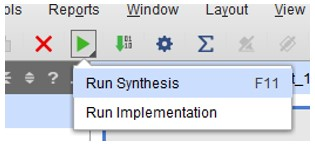
\includegraphics[width=0.5\textwidth]{fig14}
    \caption{Running synthesis}
    \label{fig:run_synthesis}
\end{figure}

Then the next window appears, indicating the completion of the synthesis stage. Now, by selecting \textbf{Run Implementation} and clicking \textbf{OK}, the implementation process begins, and again we must wait until it is completed (Figure~\ref{fig:run_implementation}).

\begin{figure}[H]
    \centering
    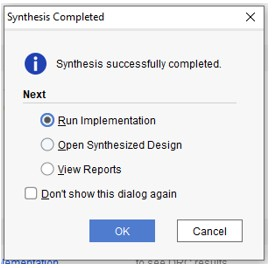
\includegraphics[width=0.5\textwidth]{fig15}
    \caption{Starting implementation after synthesis}
    \label{fig:run_implementation}
\end{figure}

After the following window appears, we select \textbf{Generate Bitstream}, and by clicking \textbf{OK}, the bitstream generation process begins (Figure~\ref{fig:generate_bitstream}).

\begin{figure}[H]
    \centering
    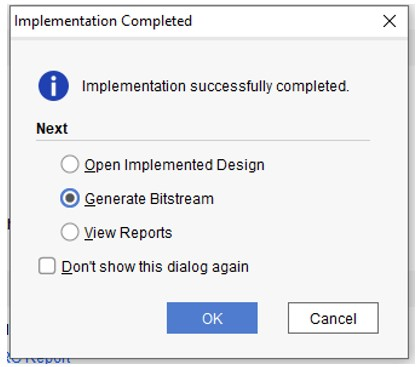
\includegraphics[width=0.5\textwidth]{fig16}
    \caption{Generating the bitstream}
    \label{fig:generate_bitstream}
\end{figure}

From the top menu bar, go to \textbf{File}, then \textbf{Export}, and click \textbf{Export Hardware} (Figure~\ref{fig:fig50}).

\begin{figure}[H]
    \centering
    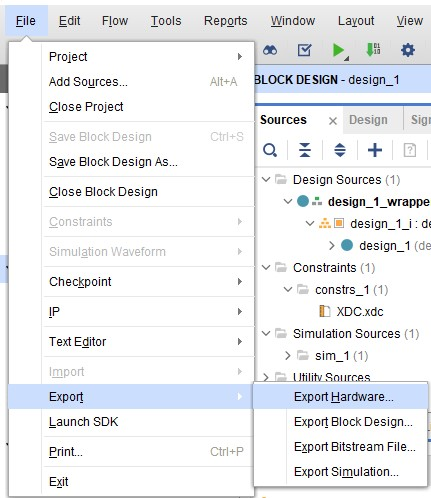
\includegraphics[width=0.5\textwidth]{fig50}
    \caption{Opening the Export Hardware option}
    \label{fig:fig50}
\end{figure}

In the displayed window, check \textbf{Include bitstream} and click \textbf{OK} (Figure~\ref{fig:fig51}).

\begin{figure}[H]
    \centering
    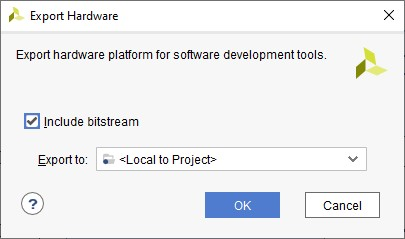
\includegraphics[width=0.5\textwidth]{fig51}
    \caption{Exporting hardware with the bitstream included}
    \label{fig:fig51}
\end{figure}


\subsubsection{Program}
From the top menu bar in Vivado, go to \textbf{File} and click \textbf{Launch SDK}.

\begin{figure}[H]
    \centering
    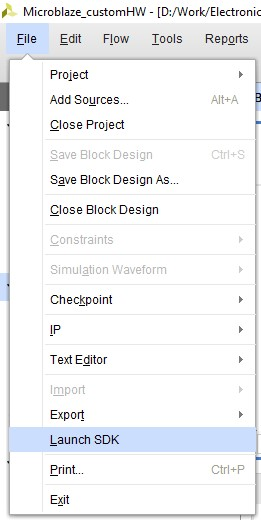
\includegraphics[width=0.5\textwidth]{fig52}
    \caption{Launching SDK from Vivado}
    \label{fig:fig52}
\end{figure}

From the top menu bar in SDK, go to \textbf{File}, then \textbf{New}, and click \textbf{Application Project}.

\begin{figure}[H]
    \centering
    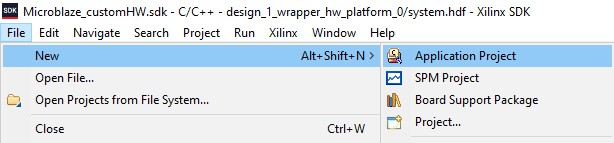
\includegraphics[width=0.5\textwidth]{fig53}
    \caption{Creating a new application project in SDK}
    \label{fig:fig53}
\end{figure}

Set a name for the project and check that the other options are the same as shown in Figure~\ref{fig:fig54}, then click \textbf{Next}.

\begin{figure}[H]
    \centering
    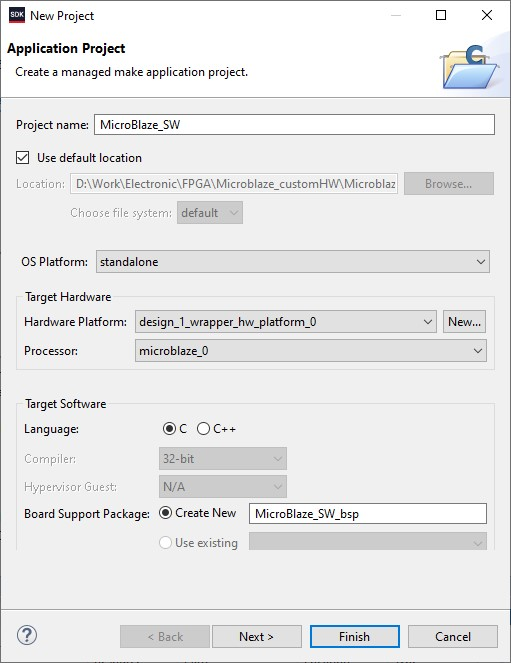
\includegraphics[width=0.5\textwidth]{fig54}
    \caption{Configuring the application project settings}
    \label{fig:fig54}
\end{figure}

Choose \textbf{Empty Application} and click \textbf{Finish} to complete the project creation process.

\begin{figure}[H]
    \centering
    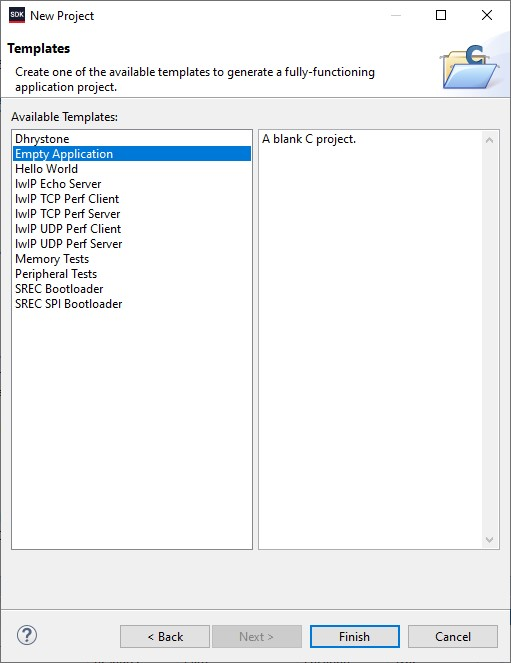
\includegraphics[width=0.5\textwidth]{fig55}
    \caption{Selecting an empty application template}
    \label{fig:fig55}
\end{figure}

In the \textbf{Project Explorer}, find the project that we just created, go to the \textbf{src} folder, and right-click on it. Then go to \textbf{New} and click \textbf{File} in order to create a new source file.

\begin{figure}[H]
    \centering
    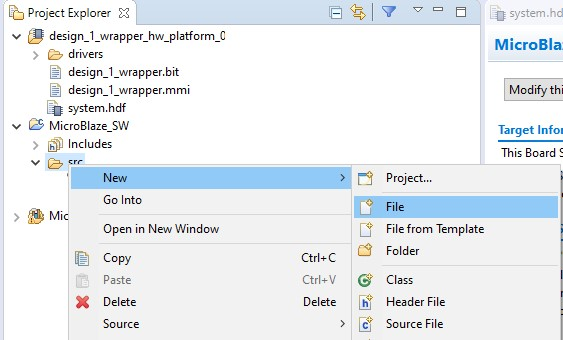
\includegraphics[width=0.5\textwidth]{fig56}
    \caption{Creating a new source file in the project}
    \label{fig:fig56}
\end{figure}

In the displayed window, enter the file name \texttt{main.c} and click \textbf{Finish}.

\begin{figure}[H]
    \centering
    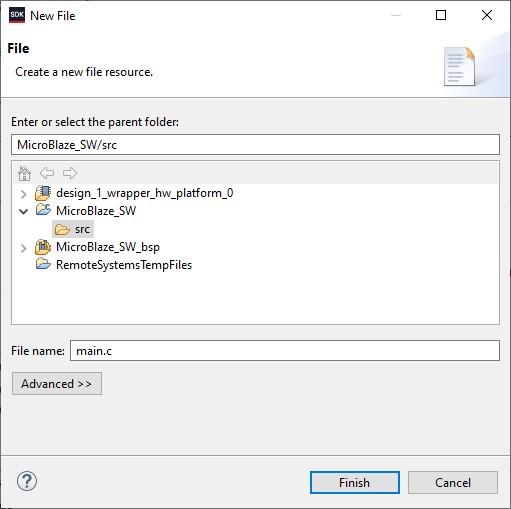
\includegraphics[width=0.5\textwidth]{fig57}
    \caption{Creating the \texttt{main.c} source file}
    \label{fig:fig57}
\end{figure}

As mentioned before, we are working with a memory-mapped system, so it is important to know and use the peripheral addresses. To access this information, there is a header file called \texttt{xparameters.h}, which contains the required definitions extracted from Vivado. This file can be accessed through \texttt{PROJECTNAME\_bsp -> microblaze\_0 -> include}. Some of the contents of this header file are shown in Figure~\ref{fig:fig58}.

\begin{figure}[H]
    \centering
    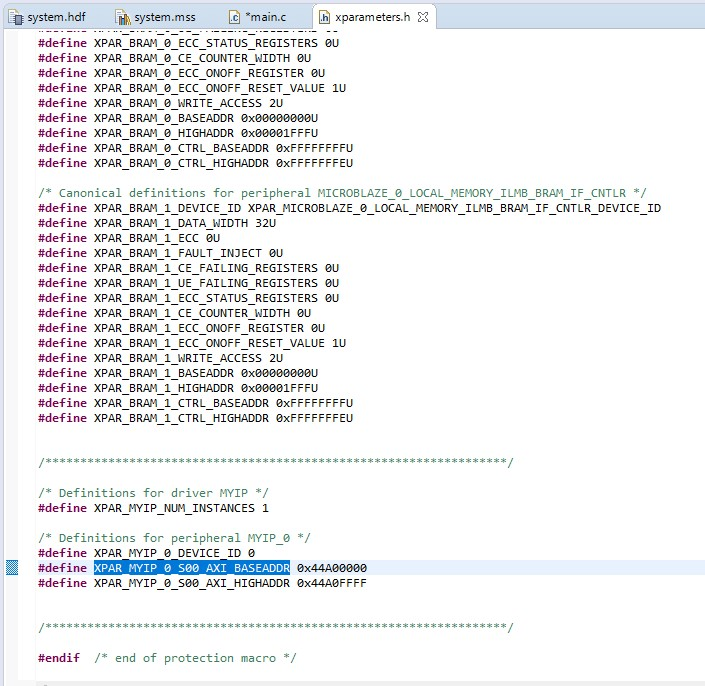
\includegraphics[width=0.5\textwidth]{fig58}
    \caption{Contents of the \texttt{xparameters.h} header file}
    \label{fig:fig58}
\end{figure}


Back in \texttt{main.c}, an example C program for the MicroBlaze processor is shown in Listing~\ref{lst:c_example}.

\begin{lstlisting}[language=C, caption={Example C program for accessing the custom IP from MicroBlaze}, label={lst:c_example}]
#include "xparameters.h"
#include "xil_io.h"
#include "xil_types.h"

int main(){
    u32 sum1, sum2;

    Xil_Out32(XPAR_MYIP_0_S00_AXI_BASEADDR, 7);
    Xil_Out32(XPAR_MYIP_0_S00_AXI_BASEADDR + 4, 5);
    sum1 = Xil_In32(XPAR_MYIP_0_S00_AXI_BASEADDR + 8);

    Xil_Out32(XPAR_MYIP_0_S00_AXI_BASEADDR, 2);
    Xil_Out32(XPAR_MYIP_0_S00_AXI_BASEADDR + 4, 1);
    sum2 = Xil_In32(XPAR_MYIP_0_S00_AXI_BASEADDR + 8);

    while(1);
    return 0;
}
\end{lstlisting}

This program demonstrates how the MicroBlaze processor communicates with the custom AXI-based IP through memory-mapped registers. The header file \texttt{xparameters.h} provides the base address of the custom peripheral, while \texttt{xil\_io.h} provides the \texttt{Xil\_Out32} and \texttt{Xil\_In32} functions for writing to and reading from hardware registers. The data type \texttt{u32}, defined in \texttt{xil\_types.h}, is used for 32-bit unsigned values.

In the first test, the values \texttt{7} and \texttt{5} are written into the first two registers of the custom IP. These correspond to the two inputs of the adder hardware. Then, the result is read from the third register and stored in \texttt{sum1}. Since the custom hardware performs addition, the expected result is \texttt{12}.

In the second test, the values \texttt{2} and \texttt{1} are written to the same input registers, and the result is again read from the output register and stored in \texttt{sum2}. In this case, the expected result is \texttt{3}.

The address offsets are important here. The base address \texttt{XPAR\_MYIP\_0\_S00\_AXI\_BASEADDR} refers to the first register. Adding an offset of \texttt{4} accesses the second 32-bit register, and adding an offset of \texttt{8} accesses the third 32-bit register. Since each register is 32 bits wide, each one occupies 4 bytes in the memory map.

Finally, the statement \texttt{while(1);} keeps the program running indefinitely so that the computed values remain available during debugging. This allows the user to inspect \texttt{sum1} and \texttt{sum2} in the debugger and verify that the software and custom hardware are working correctly together.

Then, we build the project, as shown in Figure~\ref{fig:fig59}.

\begin{figure}[H]
    \centering
    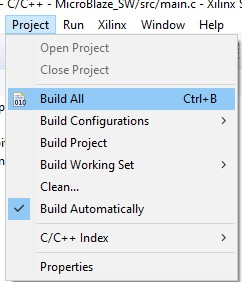
\includegraphics[width=0.5\textwidth]{fig59}
    \caption{Building the application project in SDK}
    \label{fig:fig59}
\end{figure}

According to our design, there are two things that must be programmed onto the chip. One is the \textbf{bitstream}, which contains the complete hardware system including MicroBlaze, custom hardware, memory, and other components. The other is the \textbf{software program}, which is executed by the MicroBlaze soft-core processor.

There are two ways to do this:

\paragraph{Option 1: Programming the Hardware in Vivado}

First, program the hardware in Vivado. Then, return to the SDK, right-click on the project, go to \textbf{Debug As}, and click \textbf{Launch on Hardware (System Debugger)}, as shown in Figure~\ref{fig:fig66}.

\begin{figure}[H]
    \centering
    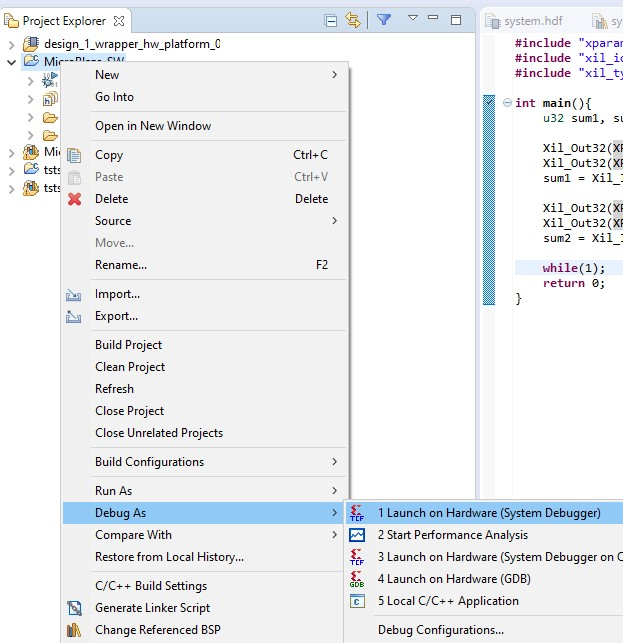
\includegraphics[width=0.5\textwidth]{fig66}
    \caption{Launching the software on hardware from SDK}
    \label{fig:fig66}
\end{figure}

\paragraph{Option 2: Using Only SDK}

Alternatively, using only the SDK, right-click on the project, go to \textbf{Debug As}, and click \textbf{Debug Configurations}. Then double-click on \textbf{Xilinx C/C++ Application (System Debugger)}, as shown in Figure~\ref{fig:fig61}.

\begin{figure}[H]
    \centering
    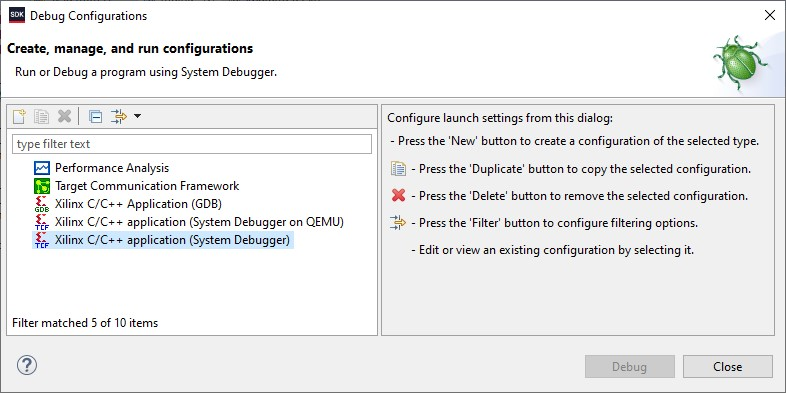
\includegraphics[width=0.5\textwidth]{fig61}
    \caption{Opening the system debugger configuration in SDK}
    \label{fig:fig61}
\end{figure}

In the opened window, under the \textbf{Target Setup} tab, choose the options exactly as shown in Figure~\ref{fig:fig62} and then click Debug.

\begin{figure}[H]
    \centering
    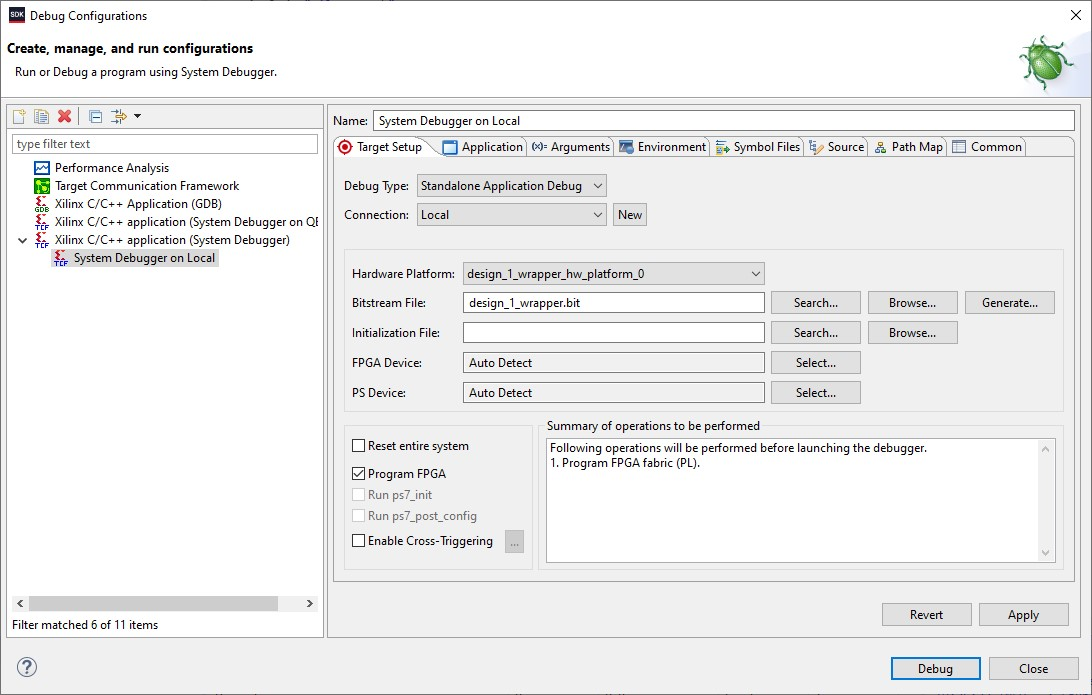
\includegraphics[width=0.5\textwidth]{fig62}
    \caption{Target setup options in the system debugger}
    \label{fig:fig62}
\end{figure}

After performing either Option 1 or Option 2, a warning message may appear. This warning is not important in this case, because we are not using the Processing System (\textbf{PS}) at this stage, as shown in Figure~\ref{fig:fig63}.

\begin{figure}[H]
    \centering
    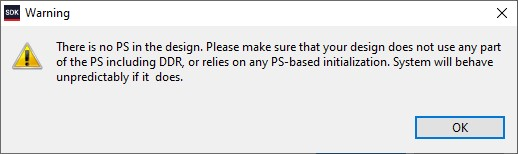
\includegraphics[width=0.5\textwidth]{fig63}
    \caption{Warning message related to the unused Processing System}
    \label{fig:fig63}
\end{figure}

After the programming process is completed, a new message appears asking whether we want to switch to the debug environment. By choosing \textbf{Yes}, we enter the debug environment.

\begin{figure}[H]
    \centering
    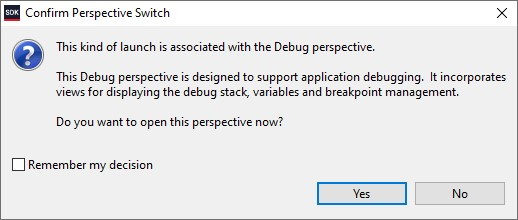
\includegraphics[width=0.5\textwidth]{fig64}
    \caption{Switching to the debug environment}
    \label{fig:fig64}
\end{figure}

After running the software completely, or step by step using the debug tools, we can observe that both the software and hardware behave as expected, as shown by the values of \texttt{sum1} and \texttt{sum2} in Figure~\ref{fig:fig65}.

\begin{figure}[H]
    \centering
    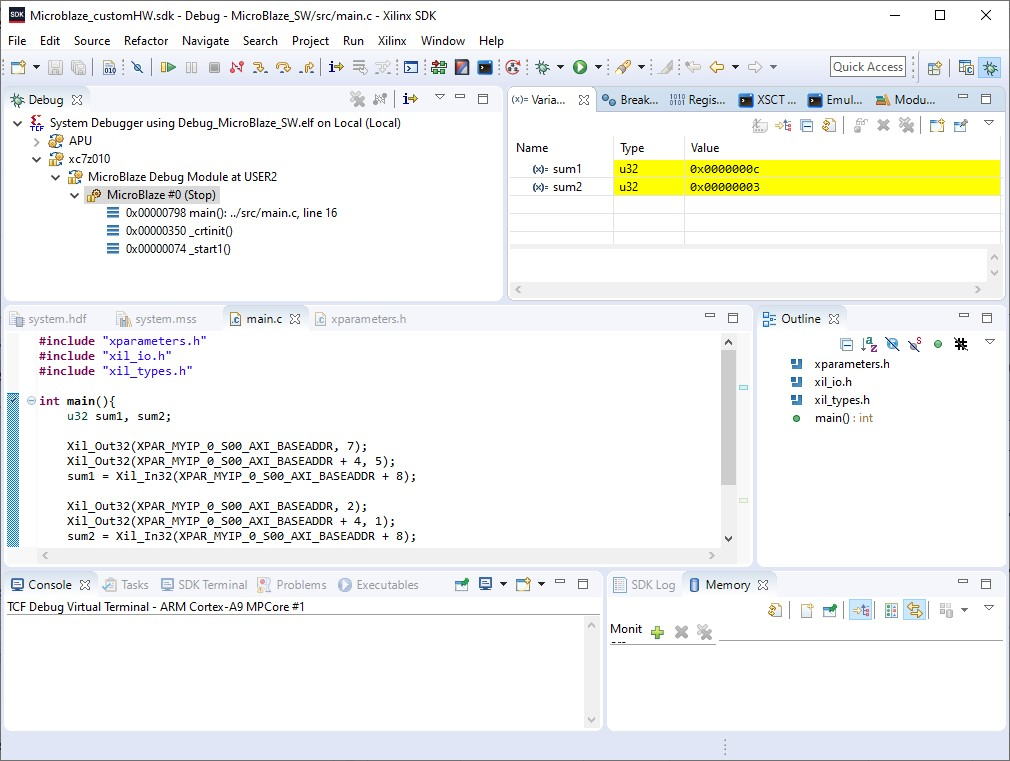
\includegraphics[width=0.5\textwidth]{fig65}
    \caption{Debug results showing correct software and hardware operation}
    \label{fig:fig65}
\end{figure}

\subsubsection{More Complex}

For a more advanced custom IP design, the simple adder can be replaced with a counter. This is beneficial because a counter includes internal state, and several configurable parameters, making it a more realistic example of a hardware peripheral. Unlike the adder, which performs only a simple combinational function, the counter demonstrates how a custom IP can support memory-mapped control registers, clock-driven operation, and multiple modes such as reset, enable, direction control, and value loading. In addition, an important feature of this design is that the 5 least significant bits (LSBs) of the counter value are displayed on the on-board LEDs. Therefore, besides the AXI interface, the custom hardware must also provide an additional output port connected directly to the LEDs.

The register map of the counter-based custom IP is shown in Table~\ref{tab:counter_register_map}. This table describes the address offsets, register names, access types, and the function of each register used to control and monitor the counter peripheral.

\begin{table}[H]
\centering
\renewcommand{\arraystretch}{1.4}
\begin{tabular}{|c|c|c|p{8.2cm}|}
\hline
\textbf{Offset} & \textbf{Name} & \textbf{Access} & \textbf{Description} \\
\hline
\texttt{0x00} & \texttt{CONTROL} & \texttt{R/W} &
\texttt{bit[0]}: \textbf{RESET}\\
&&&
\texttt{bit[1]}: \textbf{ENABLE}\\
&&&
\texttt{bit[2]}: \textbf{DIR} (0 = up, 1 = down)\\
&&&
\texttt{bit[3]}: \textbf{LOAD}\\
&&&
\texttt{bit[31:4]}: Reserved
\\
\hline
\texttt{0x04} & \texttt{PERIOD} & \texttt{R/W} &
Divider period value. The counter updates once every \texttt{PERIOD+1} clock cycles.
\\
\hline
\texttt{0x08} & \texttt{COUNT} & \texttt{R} &
Current value of the visible counter \texttt{cnt}.
\\
\hline
\texttt{0x0C} & \texttt{LOAD\_VALUE} & \texttt{R/W} &
Value written into \texttt{cnt} when \texttt{CONTROL.LOAD} is asserted.
\\
\hline
\end{tabular}
\caption{Register map of the counter-based custom IP}
\label{tab:counter_register_map}
\end{table}


The steps are similar to the previous example, so here we focus only on the required code changes. After adding MicroBlaze and the other required components to the block design, we create a custom IP called \texttt{mycounter} with an AXI Lite slave interface. Then, we go to the source file \texttt{mycounter\_v1\_0\_S00\_AXI.v}. In the module ports, we add a 5-bit output wire as shown in Listing~\ref{lst:counter_port}.

\begin{lstlisting}[language=Verilog, caption={Adding the LED output port to the custom counter IP}, label={lst:counter_port}]
...
    // Users to add ports here
    output wire [4:0] led_out,
    // User ports ends
...
\end{lstlisting}

Further in the code, in the AXI read logic, we replace \texttt{slv\_reg2} with \texttt{cnt}, so that the processor reads the current counter value instead of a standard slave register, as shown in Listing~\ref{lst:counter_read_logic}.

\begin{lstlisting}[language=Verilog, caption={Modifying the AXI read logic to return the counter value}, label={lst:counter_read_logic}]
...
      // Address decoding for reading registers
      case ( axi_araddr[ADDR_LSB+OPT_MEM_ADDR_BITS:ADDR_LSB] )
        2'h0   : reg_data_out <= slv_reg0;
        2'h1   : reg_data_out <= slv_reg1;
        2'h2   : reg_data_out <= cnt; 	//Changed
        2'h3   : reg_data_out <= slv_reg3;
        default : reg_data_out <= 0;
      endcase
...
\end{lstlisting}

Finally, we add the main counter logic in the appropriate user logic section, as shown in Listing~\ref{lst:counter_logic}.

\begin{lstlisting}[language=Verilog, caption={User logic for the AXI-based counter with LED output}, label={lst:counter_logic}]
...
// Add user logic here
reg [31:0] div_cnt;
reg [31:0] cnt;

always @(posedge S_AXI_ACLK) begin
    if (!S_AXI_ARESETN) begin
        div_cnt <= 32'd0;
        cnt     <= 32'd0;
    end
    else if (slv_reg0[0]) begin
        // software reset
        div_cnt <= 32'd0;
        cnt     <= 32'd0;
    end
    else if (slv_reg0[3]) begin
        // software load
        div_cnt <= 32'd0;
        cnt     <= slv_reg3;
    end
    else if (slv_reg0[1]) begin
        // enable
        if (div_cnt >= slv_reg1) begin
            div_cnt <= 32'd0;

            if (slv_reg0[2] == 1'b0) begin
                // up
                cnt <= cnt + 1'b1;
            end
            else begin
                // down
                cnt <= cnt - 1'b1;
            end
        end
        else begin
            div_cnt <= div_cnt + 1'b1;
        end
    end
end

assign led_out = cnt[4:0];
// User logic ends
...
\end{lstlisting}

In this design, \texttt{slv\_reg0} is used as the control register. Its bits determine whether the counter is reset, enabled, loaded with a new value, or operated in the up-counting or down-counting mode. The register \texttt{slv\_reg1} stores the divider period, which controls how often the visible counter value is updated. The register \texttt{slv\_reg3} is used as the load value, and the internal register \texttt{cnt} stores the current counter value. In addition, the signal \texttt{led\_out} is assigned to the 5 least significant bits of \texttt{cnt}, so the current counter value can be observed directly on the board LEDs.
Because we are adding a new port, we must also modify the top-level module. For this purpose, open the top-level Verilog source file, which is usually named \texttt{mycounter\_v1\_0.v}. In the port section, add the new output port in an appropriate place, as shown in Listing~\ref{lst:mycounter_top_port}.

\begin{lstlisting}[language=Verilog, caption={Adding the LED output port to the top-level custom IP module}, label={lst:mycounter_top_port}]
...
    // Users to add ports here
    output wire [4:0] led_out,
    // User ports ends
...
\end{lstlisting}

We also need to modify the instantiated AXI module further below in the same file and connect the new port, as shown in Listing~\ref{lst:mycounter_top_inst}.

\begin{lstlisting}[language=Verilog, caption={Connecting the LED output port in the top-level module instance}, label={lst:mycounter_top_inst}]
...
) mycounter_v1_0_S00_AXI_inst (
    .led_out(led_out),
    .S_AXI_ACLK(s00_axi_aclk),
...
\end{lstlisting}

After updating, upgrading, and re-packaging the custom IP, the final block design should be as shown in Figure~\ref{fig:fig67}.

\begin{figure}[H]
    \centering
    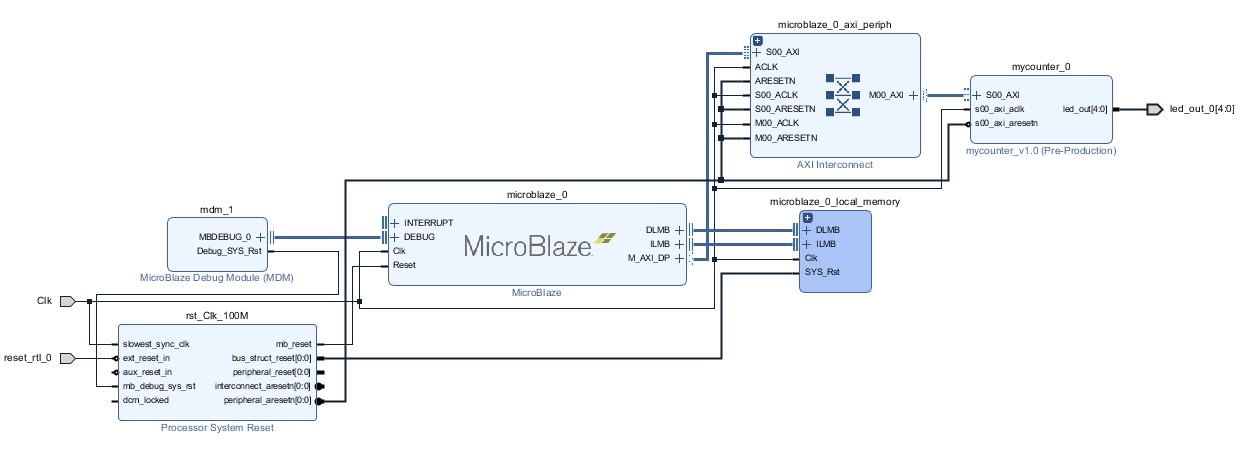
\includegraphics[width=0.8\textwidth]{fig67}
    \caption{Final block design of the counter-based system}
    \label{fig:fig67}
\end{figure}

We should also add a constraint file and assign the external pins for the clock, reset, and LED outputs, as shown in Figure~\ref{fig:fig67} and Listing~\ref{lst:mycounter_xdc}.

\begin{lstlisting}[caption={Constraint file for clock, reset, and LED pin assignment}, label={lst:mycounter_xdc}]
set_property PACKAGE_PIN U19 [get_ports reset_rtl_0]
set_property IOSTANDARD LVCMOS33 [get_ports reset_rtl_0]

set_property PACKAGE_PIN U18 [get_ports Clk]
set_property IOSTANDARD LVCMOS33 [get_ports Clk]

set_property IOSTANDARD LVCMOS33 [get_ports {led_out_0[0]}]
set_property PACKAGE_PIN V20 [get_ports {led_out_0[0]}]

set_property IOSTANDARD LVCMOS33 [get_ports {led_out_0[1]}]
set_property PACKAGE_PIN W19 [get_ports {led_out_0[1]}]

set_property IOSTANDARD LVCMOS33 [get_ports {led_out_0[2]}]
set_property PACKAGE_PIN W18 [get_ports {led_out_0[2]}]

set_property IOSTANDARD LVCMOS33 [get_ports {led_out_0[3]}]
set_property PACKAGE_PIN V18 [get_ports {led_out_0[3]}]

set_property IOSTANDARD LVCMOS33 [get_ports {led_out_0[4]}]
set_property PACKAGE_PIN V17 [get_ports {led_out_0[4]}]
\end{lstlisting}

After finishing the hardware design, generating the bitstream, and exporting the hardware, we can open the SDK, create a software project, and use the following C code on the MicroBlaze processor, as shown in Listing~\ref{lst:mycounter_c_example}.

\begin{lstlisting}[language=C, caption={Example C program for controlling the custom counter IP from MicroBlaze}, label={lst:mycounter_c_example}]
#include "xparameters.h"
#include "xil_io.h"
#include "xil_types.h"

#define BASE XPAR_MYCOUNTER_0_S00_AXI_BASEADDR

#define CTRL_RESET  1
#define CTRL_ENABLE 2
#define CTRL_DIR    4
#define CTRL_LOAD   8

void set_period(u32 p)      { Xil_Out32(BASE + 4, p); }
u32  read_counter(void)     { return Xil_In32(BASE + 8); }

void reset_counter(void)
{
    u32 c = Xil_In32(BASE + 0);
    Xil_Out32(BASE + 0, c | CTRL_RESET);
    Xil_Out32(BASE + 0, c & ~CTRL_RESET);
}

void load_counter(u32 v)
{
    u32 c = Xil_In32(BASE + 0);
    Xil_Out32(BASE + 12, v);
    Xil_Out32(BASE + 0, c | CTRL_LOAD);
    Xil_Out32(BASE + 0, c & ~CTRL_LOAD);
}

void set_up(void)           { Xil_Out32(BASE + 0, Xil_In32(BASE + 0) & ~CTRL_DIR); }
void start_counter(void)    { Xil_Out32(BASE + 0, Xil_In32(BASE + 0) |  CTRL_ENABLE); }
void stop_counter(void)     { Xil_Out32(BASE + 0, Xil_In32(BASE + 0) & ~CTRL_ENABLE); }

int main(void)
{
    u32 c0, c1;

    reset_counter();
    set_period(25000000);
    load_counter(2);
    set_up();
    start_counter();

    c0 = read_counter();
    c1 = read_counter();

    while (1);
    return 0;
}
\end{lstlisting}

This software demonstrates how the MicroBlaze processor controls the custom counter IP through its memory-mapped AXI registers. The base address of the peripheral is defined by \texttt{XPAR\_MYCOUNTER\_0\_S00\_AXI\_BASEADDR}, which is provided in the \texttt{xparameters.h} header file. The software uses \texttt{Xil\_Out32} to write values into the counter registers and \texttt{Xil\_In32} to read values back.

The control register is located at offset \texttt{0x00}. Several bit masks are defined for this register: \texttt{CTRL\_RESET} resets the counter, \texttt{CTRL\_ENABLE} enables counting, \texttt{CTRL\_DIR} selects the counting direction, and \texttt{CTRL\_LOAD} loads a predefined value into the counter. The function \texttt{set\_period()} writes the divider period to offset \texttt{0x04}, while \texttt{read\_counter()} reads the current counter value from offset \texttt{0x08}.

The function \texttt{reset\_counter()} performs a software reset by setting and then clearing the reset bit in the control register. Similarly, \texttt{load\_counter()} writes a value to the load register at offset \texttt{0x0C}, then pulses the load bit so that the counter is initialized with the requested value. The functions \texttt{set\_up()}, \texttt{start\_counter()}, and \texttt{stop\_counter()} configure the counter direction and control whether the counting process is active.

In the \texttt{main()} function, the counter is first reset, then its update period is set to \texttt{25000000}. After that, the value \texttt{2} is loaded into the counter, the counting direction is set to up-counting, and the counter is started. The variables \texttt{c0} and \texttt{c1} store values read from the counter and can be inspected in the debugger. At the same time, the 5 least significant bits of the counter value are continuously driven to the board LEDs through the \texttt{led\_out} port, allowing the counter operation to be observed directly in hardware.

\subsection{MicroBlaze and GPIO}

In this section, we want to work with input and output using the MicroBlaze soft-core processor. In our scenario, we use 3 input signals so that each one turns on its corresponding output LED.

After adding MicroBlaze and connecting the corresponding clock and reset signals in the block design, search for \textbf{AXI GPIO} and add it to the design block (Figure~\ref{fig:fig68}). For simplicity, we use two AXI GPIO IPs: one configured as input only and the other configured as output only\footnote{It is also possible to use a single AXI GPIO IP for both input and output.}.

\begin{figure}[H]
    \centering
    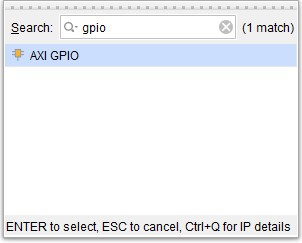
\includegraphics[width=0.5\textwidth]{fig68}
    \caption{Adding AXI GPIO IPs to the block design}
    \label{fig:fig68}
\end{figure}

Double-click on one of them to open its properties and activate the \textbf{All Inputs} checkbox. Set the GPIO width to 3 bits and make sure that \textbf{Enable Dual Channel} is unchecked (Figure~\ref{fig:fig69}). Do the same for the other AXI GPIO, but this time choose \textbf{All Outputs}.

\begin{figure}[H]
    \centering
    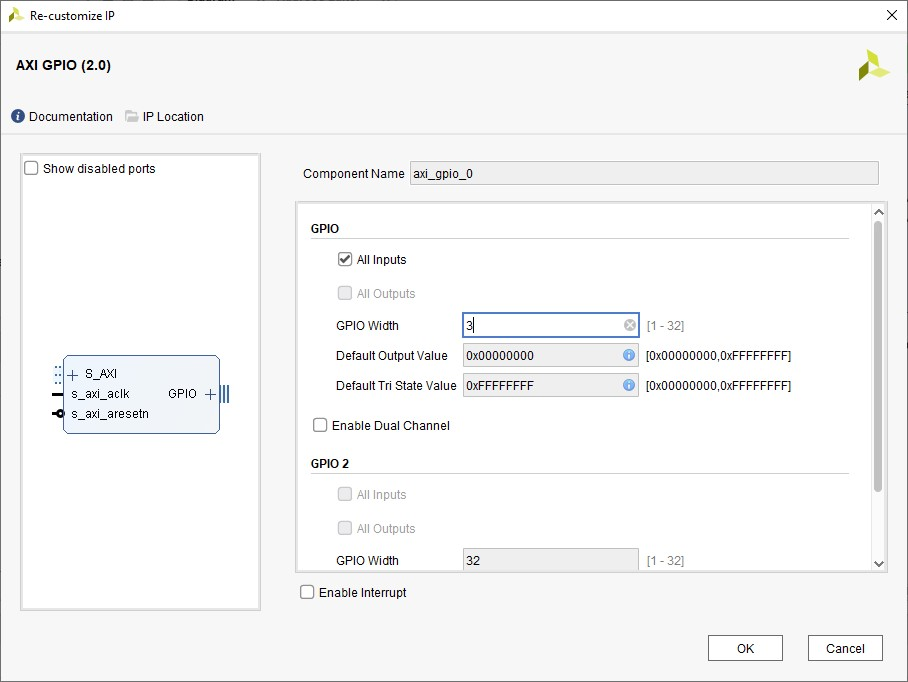
\includegraphics[width=0.5\textwidth]{fig69}
    \caption{Configuring AXI GPIO properties}
    \label{fig:fig69}
\end{figure}

For each AXI GPIO, expand the GPIO port in the block design, select the expanded port, right-click on it, and choose \textbf{Make External} (Figure~\ref{fig:fig70}). By doing this, these AXI GPIO ports are connected to the real device I/O pins.

\begin{figure}[H]
    \centering
    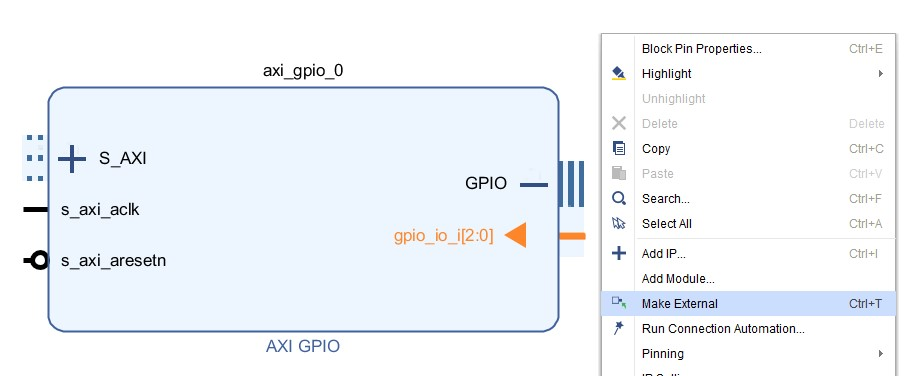
\includegraphics[width=0.5\textwidth]{fig70}
    \caption{Making the GPIO ports external}
    \label{fig:fig70}
\end{figure}

Therefore, the final block design should be as shown in Figure~\ref{fig:fig71}.

\begin{figure}[H]
    \centering
    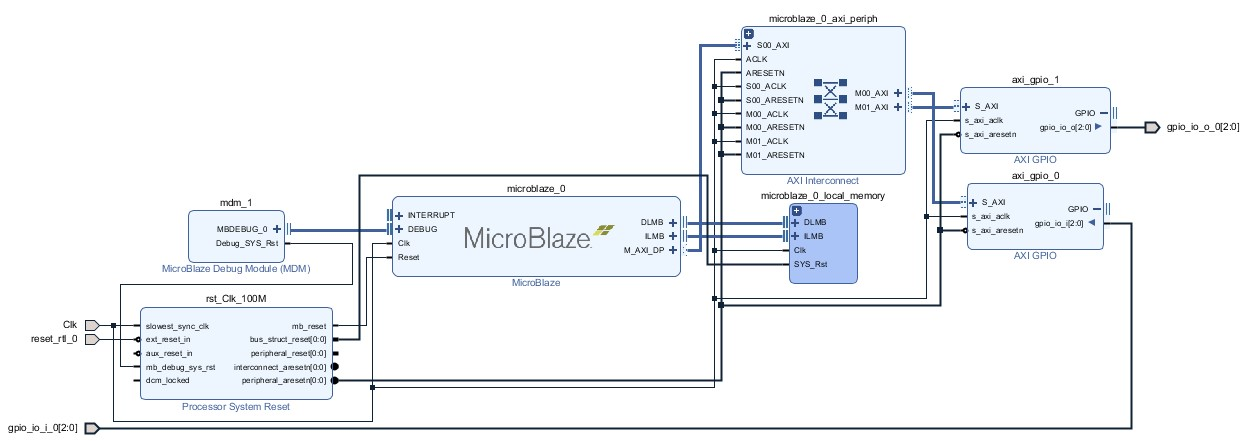
\includegraphics[width=0.5\textwidth]{fig71}
    \caption{Final block design for the MicroBlaze and GPIO system}
    \label{fig:fig71}
\end{figure}

Now it is time to assign constraints for the external ports and signals. Since the push-buttons on our development board are connected as shown in Figure~\ref{fig:fig72}, the constraint file should be written as shown in Listing~\ref{lst:gpio_xdc}.

\begin{figure}[H]
    \centering
    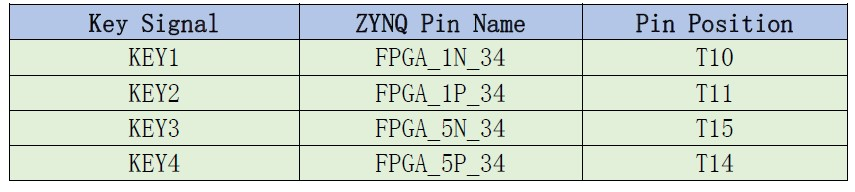
\includegraphics[width=0.5\textwidth]{fig72}
    \caption{Board pin connections for the input buttons}
    \label{fig:fig72}
\end{figure}

\begin{lstlisting}[caption={Constraint file for clock, reset, GPIO outputs, and GPIO inputs}, label={lst:gpio_xdc}]
set_property PACKAGE_PIN U19 [get_ports reset_rtl_0]
set_property IOSTANDARD LVCMOS33 [get_ports reset_rtl_0]

set_property PACKAGE_PIN U18 [get_ports Clk]
set_property IOSTANDARD LVCMOS33 [get_ports Clk]

set_property IOSTANDARD LVCMOS33 [get_ports {gpio_io_o_0[0]}]
set_property PACKAGE_PIN V20 [get_ports {gpio_io_o_0[0]}]

set_property IOSTANDARD LVCMOS33 [get_ports {gpio_io_o_0[1]}]
set_property PACKAGE_PIN W19 [get_ports {gpio_io_o_0[1]}]

set_property IOSTANDARD LVCMOS33 [get_ports {gpio_io_o_0[2]}]
set_property PACKAGE_PIN W18 [get_ports {gpio_io_o_0[2]}]

set_property IOSTANDARD LVCMOS33 [get_ports {gpio_io_i_0[0]}]
set_property PACKAGE_PIN T10 [get_ports {gpio_io_i_0[0]}]

set_property IOSTANDARD LVCMOS33 [get_ports {gpio_io_i_0[1]}]
set_property PACKAGE_PIN T11 [get_ports {gpio_io_i_0[1]}]

set_property IOSTANDARD LVCMOS33 [get_ports {gpio_io_i_0[2]}]
set_property PACKAGE_PIN T15 [get_ports {gpio_io_i_0[2]}]
\end{lstlisting}

After creating an HDL wrapper by right-clicking on the block design in the \textbf{Sources} section and choosing \textbf{Create HDL Wrapper}, we synthesize, implement, and generate the bitstream for the whole design, and finally export the hardware. Then we open the SDK, create a software project, and use the following C code on the MicroBlaze processor, as shown in Listing~\ref{lst:gpio_c_example}.

\begin{lstlisting}[language=C, caption={Example C program for controlling LEDs with buttons using AXI GPIO}, label={lst:gpio_c_example}]
#include "xparameters.h"
#include "xgpio.h"

#define LED_GPIO_ID XPAR_AXI_GPIO_1_DEVICE_ID
#define BTN_GPIO_ID XPAR_AXI_GPIO_0_DEVICE_ID

XGpio LedGpio;
XGpio BtnGpio;

int main(void)
{
    u32 btn;
    u32 led;

    XGpio_Initialize(&LedGpio, LED_GPIO_ID);
    XGpio_Initialize(&BtnGpio, BTN_GPIO_ID);

    XGpio_SetDataDirection(&LedGpio, 1, 0x0); // LEDs = output
    XGpio_SetDataDirection(&BtnGpio, 1, 0x7); // buttons = input

    while (1)
    {
        btn = XGpio_DiscreteRead(&BtnGpio, 1);
        led = 0;

        if ((btn & 0x1) == 0) led |= 0x1; // button 1 -> LED 1
        if ((btn & 0x2) == 0) led |= 0x2; // button 2 -> LED 2
        if ((btn & 0x4) == 0) led |= 0x4; // button 3 -> LED 3

        XGpio_DiscreteWrite(&LedGpio, 1, led);
    }

    return 0;
}
\end{lstlisting}

The C program in Listing~\ref{lst:gpio_c_example} shows how the MicroBlaze processor communicates with external inputs and outputs through two AXI GPIO peripherals. One AXI GPIO IP is used for the LEDs and the other is used for the buttons. In this design, the processor continuously reads the state of the push-buttons and then updates the LEDs so that each pressed button turns on its corresponding LED.

The header file \texttt{xparameters.h} contains hardware-dependent constants automatically generated from the Vivado design. These constants include the device IDs of the AXI GPIO peripherals, which are required in software to identify the correct hardware blocks. The header file \texttt{xgpio.h} provides the GPIO driver and the related functions used to initialize, configure, read, and write the GPIO modules.

The following definitions assign readable names to the two GPIO peripherals:
\texttt{LED\_GPIO\_ID} refers to the AXI GPIO connected to the LEDs, and \texttt{BTN\_GPIO\_ID} refers to the AXI GPIO connected to the buttons. Two variables of type \texttt{XGpio}, namely \texttt{LedGpio} and \texttt{BtnGpio}, are then declared. These variables are software driver instances that represent the two AXI GPIO hardware modules inside the program.

Inside the \texttt{main()} function, the variables \texttt{btn} and \texttt{led} are declared as 32-bit unsigned integers. The variable \texttt{btn} stores the value read from the button inputs, while \texttt{led} stores the value that will be written to the LED outputs.

The function \texttt{XGpio\_Initialize()} is used first for both GPIO instances. This function connects each software GPIO object to its corresponding hardware peripheral using the device ID defined in \texttt{xparameters.h}. Without this initialization step, the software would not be able to access the GPIO hardware correctly.

After initialization, the direction of each GPIO channel is configured using \texttt{XGpio\_SetDataDirection()}. This is one of the most important I/O-related functions in the code. In the AXI GPIO driver, a direction bit value of \texttt{1} means input, while a direction bit value of \texttt{0} means output. Therefore, \texttt{0x0} configures all bits of the LED GPIO as outputs, and \texttt{0x7} configures the lowest three bits of the button GPIO as inputs. Since the design uses a single channel for each GPIO, channel number 1 is used in both cases.

After the GPIO configuration is completed, the program enters an infinite \texttt{while(1)} loop. This means the processor continuously polls the buttons and updates the LEDs in real time. No interrupt mechanism is used here; instead, the processor repeatedly checks the input values by software.

The function \texttt{XGpio\_DiscreteRead()} reads the current logic value of the selected GPIO channel. In this code, it reads the state of the three push-buttons from the input AXI GPIO and stores the result in the variable \texttt{btn}. After that, the variable \texttt{led} is reset to zero so that all LED bits are initially turned off before checking the input conditions.

The three \texttt{if} statements then examine the three least significant bits of \texttt{btn}. Each statement checks one button by using a bitwise AND operation. If the corresponding button is pressed, the related LED bit is set in the variable \texttt{led}. An important detail is that the buttons are active-low. This means that when a button is pressed, its input value becomes logic 0, not logic 1. For this reason, the program checks whether each masked bit is equal to zero. If bit 0 is zero, LED 0 is turned on; if bit 1 is zero, LED 1 is turned on; and if bit 2 is zero, LED 2 is turned on.

Finally, the function \texttt{XGpio\_DiscreteWrite()} writes the value stored in \texttt{led} to the output AXI GPIO connected to the LEDs. This causes the physical LEDs on the board to turn on or off according to the button states. Therefore, the software implements a direct relation between the three input buttons and the three output LEDs.

In summary, the I/O-related functions used in this program are:
\texttt{XGpio\_Initialize()}, which initializes the GPIO driver instance;
\texttt{XGpio\_SetDataDirection()}, which configures each GPIO bit as input or output;
\texttt{XGpio\_DiscreteRead()}, which reads the current input values from a GPIO channel; and
\texttt{XGpio\_DiscreteWrite()}, which sends output values to a GPIO channel.

Overall, this example demonstrates a simple polling-based GPIO control system using MicroBlaze. The processor continuously samples the button inputs and updates the LEDs accordingly, showing how software running on MicroBlaze can interact with real external hardware through AXI GPIO peripherals.

\section{PS Only}

\section{PL - PS}

\section{Others}

\subsection{Introduction to the Xilinx System Debugger (XSDB) Tool}

This tool can be used to check the hardware connection between the board and the computer. To run this tool, as shown in the displayed path, we execute the \texttt{xsdb.bat} file.

\begin{figure}[H]
    \centering
    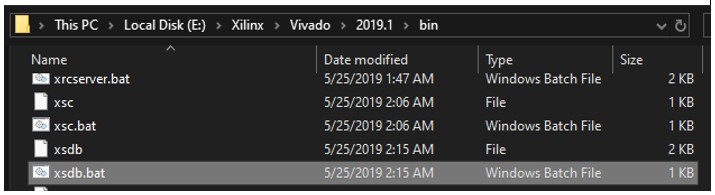
\includegraphics[width=0.5\textwidth]{fig21}
    \caption{Running the XSDB tool}
    \label{fig:run_xsdb}
\end{figure}

Then, in the opened window, the desired command can be entered.

\begin{figure}[H]
    \centering
    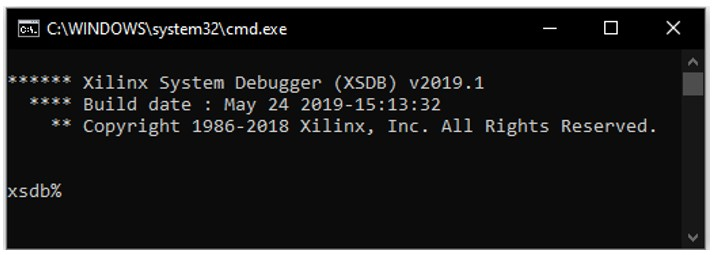
\includegraphics[width=0.5\textwidth]{fig22}
    \caption{XSDB command window}
    \label{fig:xsdb_command_window}
\end{figure}

By entering the \texttt{help} command, access to the guide for other commands is provided.

\begin{figure}[H]
    \centering
    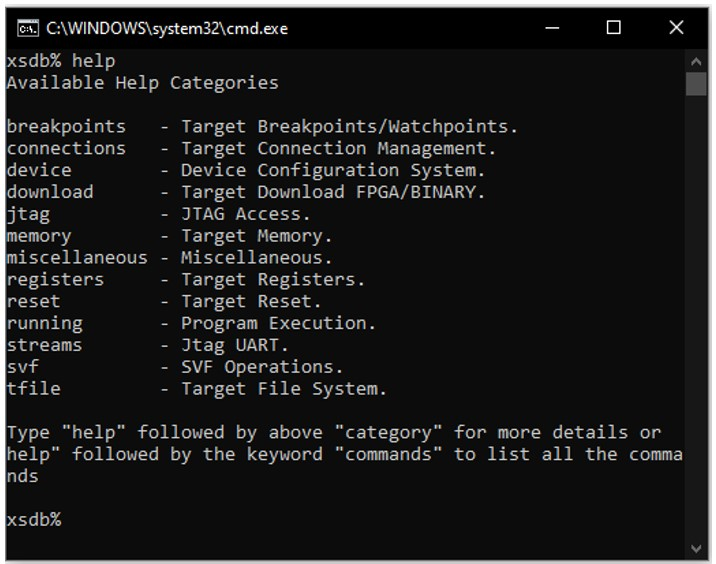
\includegraphics[width=0.5\textwidth]{fig23}
    \caption{Help command in XSDB}
    \label{fig:xsdb_help}
\end{figure}

One of the capabilities of this tool is reading from and writing to the on-chip memory (\textbf{OCM}). First, after connecting the board to the computer through the \textbf{JTAG} port, it is necessary to enter the \texttt{connect} command so that communication between the computer and the board is established. Then, by entering the \texttt{targets} command, the programmable elements available on the chip can be observed.

\begin{figure}[H]
    \centering
    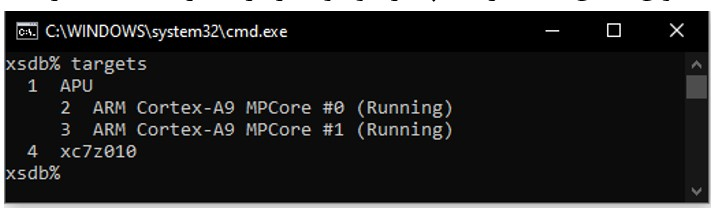
\includegraphics[width=0.5\textwidth]{fig24}
    \caption{Connecting to the board and displaying available targets}
    \label{fig:xsdb_targets}
\end{figure}

According to the figure above, it can be seen that two ARM processors and one FPGA have been recognized, which matches the chip used in this project (\textbf{Zynq7010}). To connect to one of the displayed units, for example to the first processor, the \texttt{target} command can be used as shown below.

\begin{lstlisting}[language=bash, caption={Selecting a target in XSDB}, label={lst:xsdb_target}]
xsdb% target 2
\end{lstlisting}

To read from a location in the on-chip memory, the \texttt{mrd} command is used as follows.

\begin{lstlisting}[language=bash, caption={Reading from on-chip memory in XSDB}, label={lst:xsdb_mrd}]
xsdb% mrd address
\end{lstlisting}

Also, to write to a memory location, the \texttt{mwr} command is used.

\begin{lstlisting}[language=bash, caption={Writing to on-chip memory in XSDB}, label={lst:xsdb_mwr}]
xsdb% mwr address value
\end{lstlisting}

The results of the above operations can be seen in the following figure.

\begin{figure}[H]
    \centering
    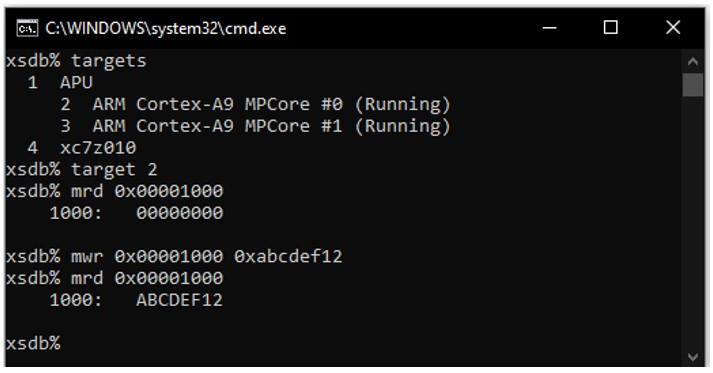
\includegraphics[width=0.5\textwidth]{fig25}
    \caption{Results of memory read and write operations in XSDB}
    \label{fig:xsdb_memory_results}
\end{figure}

According to the results, it can be observed that at address \texttt{0x00001000}, the initial value is \texttt{0x00000000}. After writing the value \texttt{0xabcdef12} to the same address and reading it again, it can be seen that the value change was successful.

\subsection{ILA (Integrated Logic Analyzer) -- Native}

In this section, we describe how to use the Integrated Logic Analyzer (ILA) to verify and debug an RTL design. Since we are not using a block design in this example, the ILA module must be instantiated directly in the Verilog design.

Assume that the project has already been created and that the following Verilog module has been designed:

\begin{lstlisting}[language=Verilog, caption={Verilog code for the LED counter design}, label={lst:ila_led_counter_original}]
`timescale 1ns / 1ps

module LED_Counter(
    input  wire clk,
    input  wire rst,
    output reg  [4:0] LED
);

reg [31:0] cnt;

always @(posedge clk) begin
    if (!rst) begin
        cnt <= 32'd0;
        LED <= 5'd0;
    end
    else begin
        if (cnt >= 32'd25_000_000 - 1) begin
            cnt <= 32'd0;
            LED <= LED + 1'b1;
        end
        else begin
            cnt <= cnt + 1'b1;
        end
    end
end

endmodule
\end{lstlisting}

From the left menu, under \textbf{Project Manager}, click on \textbf{IP Catalog}. In the IP Catalog tab, a list of available Vivado IPs is shown. Search for \textbf{ILA} as shown in Figure~\ref{fig:fig74}.

\begin{figure}[H]
    \centering
    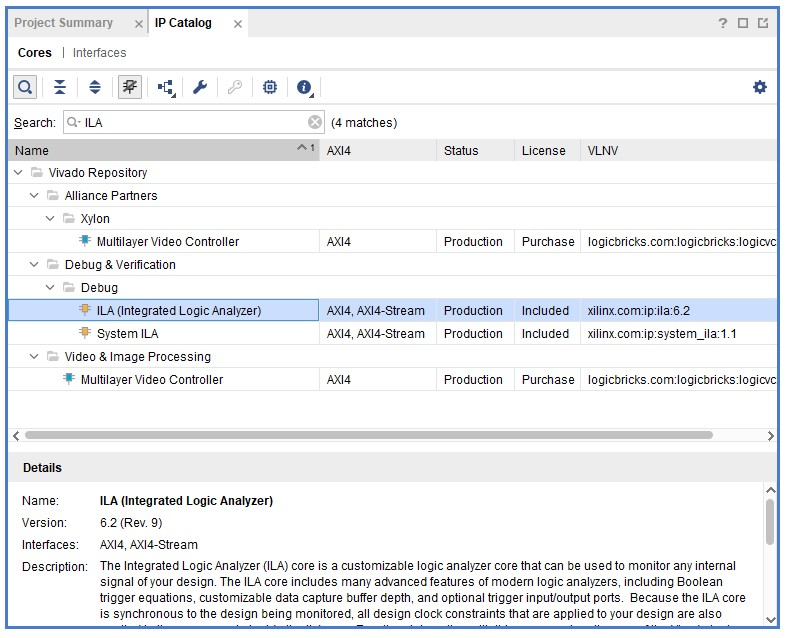
\includegraphics[width=0.5\textwidth]{fig74}
    \caption{Searching for the ILA IP in the Vivado IP Catalog}
    \label{fig:fig74}
\end{figure}

Double-click on the ILA IP. The \textbf{Customize IP} window will appear. In the general options, since we are using a purely RTL design and not an AXI interconnect, we choose the \textbf{Native} option. Because we want to monitor the signals \texttt{rst}, \texttt{cnt}, and \texttt{LED}, we set the number of probes to 3. We also set the sample data depth to 1024, or any other value as needed (Figure~\ref{fig:fig75}).

\begin{figure}[H]
    \centering
    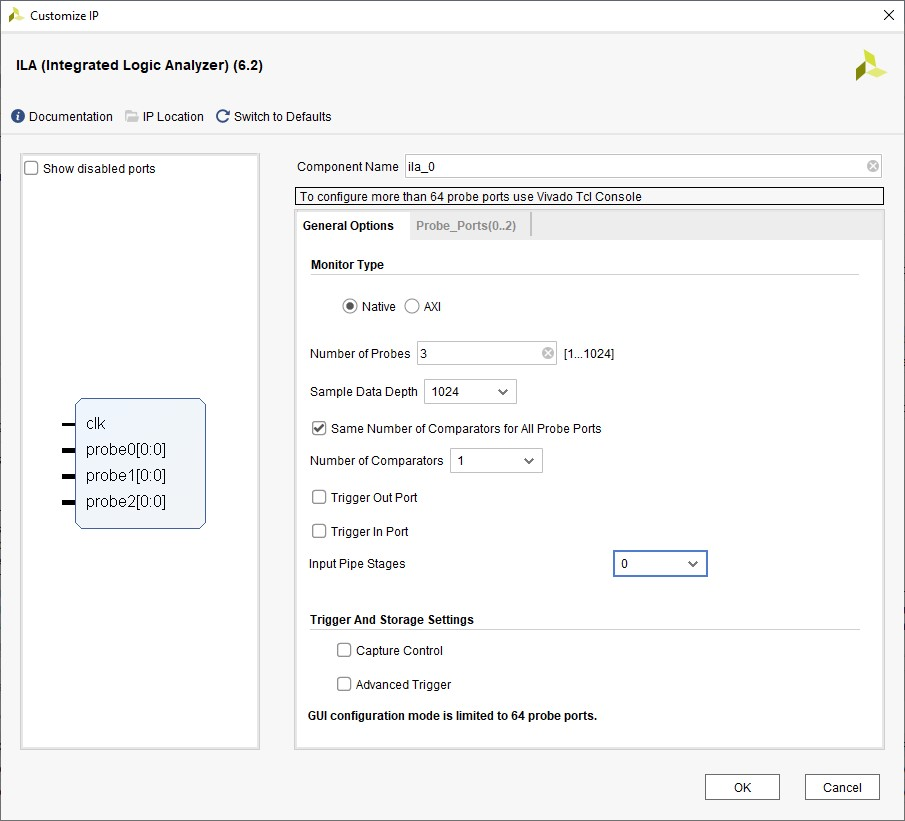
\includegraphics[width=0.5\textwidth]{fig75}
    \caption{Configuring the ILA IP in Native mode}
    \label{fig:fig75}
\end{figure}

In the \textbf{Probe Ports} tab, we set the width of each probe according to the corresponding signal width. In this example, we connect \texttt{probe0}, \texttt{probe1}, and \texttt{probe2} to \texttt{rst}, \texttt{cnt}, and \texttt{LED}, respectively. Therefore, their widths must be set to 1, 32, and 5 bits, as shown in Figure~\ref{fig:fig76}.

\begin{figure}[H]
    \centering
    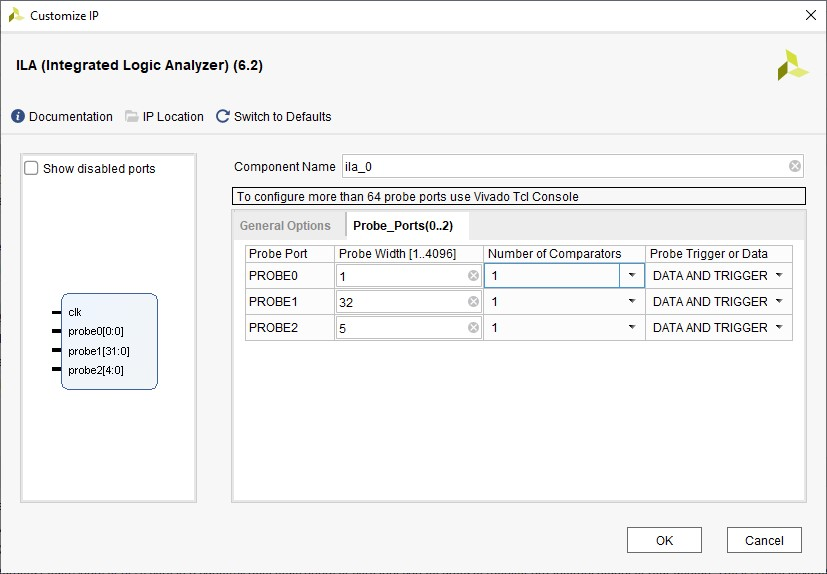
\includegraphics[width=0.5\textwidth]{fig76}
    \caption{Setting the widths of the ILA probes}
    \label{fig:fig76}
\end{figure}

After clicking \textbf{OK}, a window may appear asking whether a related directory should be created. By clicking \textbf{OK} again, the customized ILA IP core is generated (Figure~\ref{fig:fig77}).

\begin{figure}[H]
    \centering
    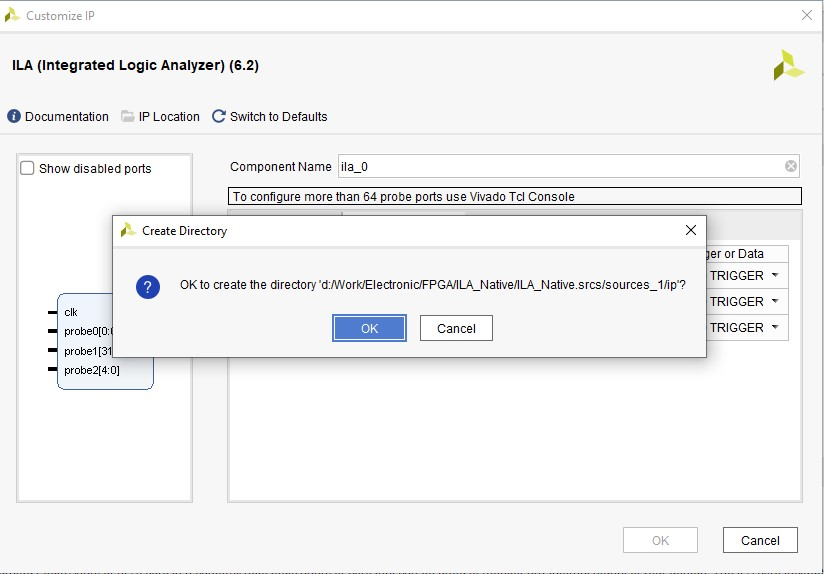
\includegraphics[width=0.5\textwidth]{fig77}
    \caption{Generating the customized ILA IP core}
    \label{fig:fig77}
\end{figure}

If a window titled \textbf{Generate Output Products} appears, click \textbf{Skip} (Figure~\ref{fig:fig78}).

\begin{figure}[H]
    \centering
    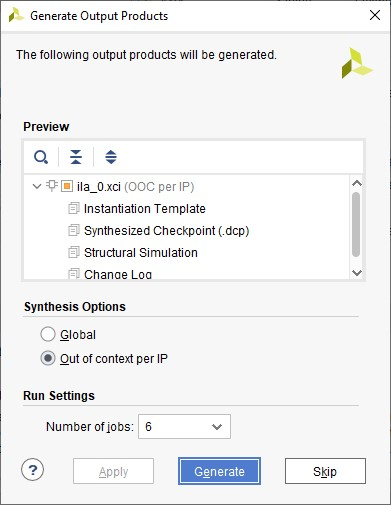
\includegraphics[width=0.5\textwidth]{fig78}
    \caption{Skipping output product generation for the ILA IP}
    \label{fig:fig78}
\end{figure}

In the \textbf{Sources} window, go to \textbf{IP Sources} and open \texttt{IP -> ila\_0 -> Instantiation Template -> ila\_0.veo} by double-clicking on it (Figure~\ref{fig:fig79}).

\begin{figure}[H]
    \centering
    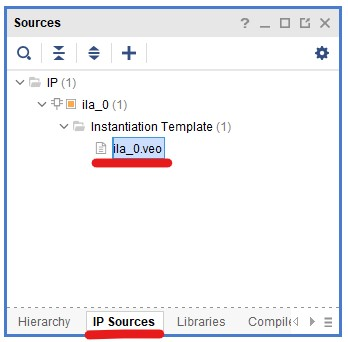
\includegraphics[width=0.5\textwidth]{fig79}
    \caption{Opening the ILA instantiation template}
    \label{fig:fig79}
\end{figure}

A window will appear that contains the ILA IP core instantiation template. We need to copy this template:

\begin{lstlisting}[language=Verilog, caption={ILA instantiation template generated by Vivado}, label={lst:ila_template}]
//----------- Begin Cut here for INSTANTIATION Template ---// INST_TAG

ila_0 your_instance_name (
    .clk(clk), // input wire clk

    .probe0(probe0), // input wire [0:0]  probe0
    .probe1(probe1), // input wire [31:0]  probe1
    .probe2(probe2)  // input wire [4:0]  probe2
);

// INST_TAG_END ------ End INSTANTIATION Template ---------
\end{lstlisting}

Then, return to the design Verilog file and paste the ILA template into it. Make sure to give the instantiated ILA a proper name and connect the correct signals to its probe ports. The final Verilog code is shown in Listing~\ref{lst:ila_led_counter_final}.

\begin{lstlisting}[language=Verilog, caption={Final Verilog design with instantiated ILA core}, label={lst:ila_led_counter_final}]
`timescale 1ns / 1ps
module LED_Counter(
    input  wire clk,
    input  wire rst,
    output reg  [4:0] LED
);
reg [31:0] cnt;
always @(posedge clk) begin
    if (!rst) begin
        cnt <= 32'd0;
        LED <= 5'd0;
    end
    else begin
        if (cnt >= 32'd25_000_000 - 1) begin
            cnt <= 32'd0;
            LED <= LED + 1'b1;
        end
        else begin
            cnt <= cnt + 1'b1;
        end
    end
end

ila_0 myila (
    .clk(clk),
    .probe0(rst),
    .probe1(cnt),
    .probe2(LED)
);
endmodule
\end{lstlisting}

Next, create a constraint file according to the FPGA development board being used:

\begin{lstlisting}[caption={Constraint file for the LED counter with ILA}, label={lst:ila_xdc}]
set_property IOSTANDARD LVCMOS33 [get_ports clk]
set_property PACKAGE_PIN U18 [get_ports clk]

set_property IOSTANDARD LVCMOS33 [get_ports {rst}]
set_property PACKAGE_PIN T10 [get_ports {rst}]

set_property IOSTANDARD LVCMOS33 [get_ports {LED[0]}]
set_property PACKAGE_PIN V20 [get_ports {LED[0]}]

set_property IOSTANDARD LVCMOS33 [get_ports {LED[1]}]
set_property PACKAGE_PIN W19 [get_ports {LED[1]}]

set_property IOSTANDARD LVCMOS33 [get_ports {LED[2]}]
set_property PACKAGE_PIN W18 [get_ports {LED[2]}]

set_property IOSTANDARD LVCMOS33 [get_ports {LED[3]}]
set_property PACKAGE_PIN V18 [get_ports {LED[3]}]

set_property IOSTANDARD LVCMOS33 [get_ports {LED[4]}]
set_property PACKAGE_PIN V17 [get_ports {LED[4]}]
\end{lstlisting}

After saving the edited file, run synthesis, implementation, and bitstream generation, and then program the chip, as shown in Figure~\ref{fig:fig80}.

\begin{figure}[H]
    \centering
    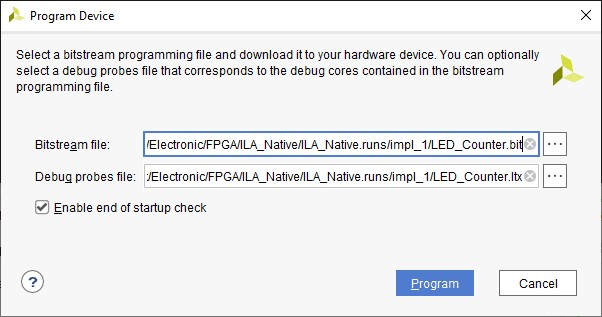
\includegraphics[width=0.5\textwidth]{fig80}
    \caption{Programming the FPGA with the design containing the ILA}
    \label{fig:fig80}
\end{figure}

After programming is completed, the ILA window opens automatically.

\begin{figure}[H]
    \centering
    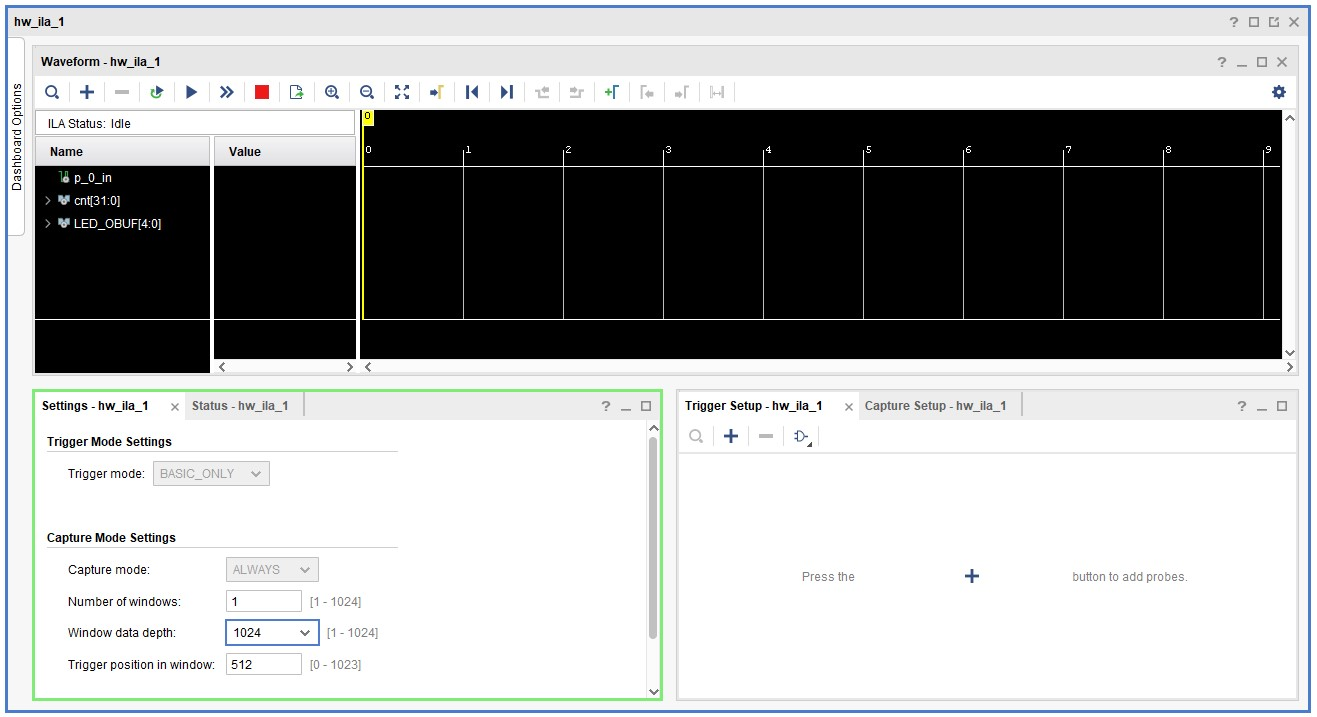
\includegraphics[width=0.5\textwidth]{fig81}
    \caption{ILA window after programming the FPGA}
    \label{fig:fig81}
\end{figure}

In the \textbf{Trigger Setup} window, a signal can be selected as the trigger condition so that the waveform is captured when the selected condition occurs. For example, we can add the reset signal (named \texttt{p\_0\_in} or a similar automatically assigned name in the ILA window) and set its trigger value to 0, because the reset button on the development board is active-low. After clicking \textbf{Run Trigger for this ILA core} and pressing the assigned reset button, the waveform can be observed as shown in Figure~\ref{fig:fig82}.

\begin{figure}[H]
    \centering
    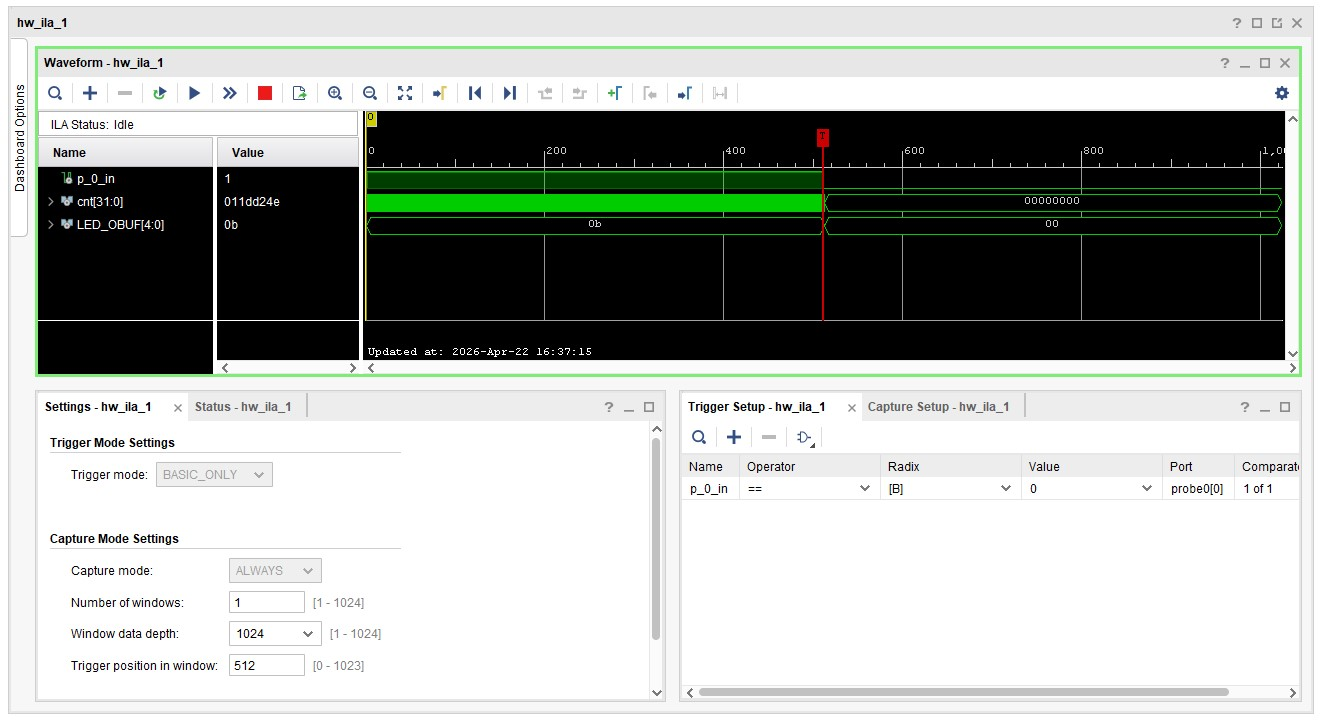
\includegraphics[width=0.5\textwidth]{fig82}
    \caption{Captured waveform in the ILA after the trigger condition is met}
    \label{fig:fig82}
\end{figure}

More trigger conditions can also be added in the \textbf{Trigger Setup} window, but in that case it is important to set the \textbf{Trigger Condition} option to \textbf{Global OR}, as shown in Figure~\ref{fig:fig83}.

\begin{figure}[H]
    \centering
    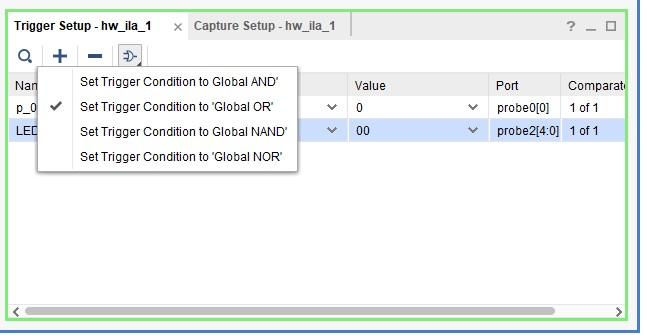
\includegraphics[width=0.5\textwidth]{fig83}
    \caption{Setting multiple trigger conditions using Global OR}
    \label{fig:fig83}
\end{figure}

Another way to capture the waveform is without defining any trigger condition. This can be done by clicking \textbf{Run Trigger Immediate for the ILA core}.
\begin{lstlisting}[language=C, caption={Example C program}, label={lst:c_example}]
#include <stdio.h>

int main() {
    int counter = 0;
    for (int i = 0; i < 10; i++) {
        counter++;
    }
    printf("Counter = %d\n", counter);
    return 0;
}
\end{lstlisting}




\end{document}